\documentclass[referee,a4paper,12pt,traditabstract]{swsc}

\usepackage{graphicx}
\usepackage{txfonts}
\usepackage{subfigure}
\usepackage{epstopdf}
\usepackage{lineno}
\usepackage[authoryear,round]{natbib}
\usepackage[backref]{hyperref}
\usepackage{url}

\author{A. Leonard \and H. Morgan}

\institute{Institute of Mathematics, Physics and Computer Science, Aberystwyth University, Ceredigion, SY23 3BZ, Wales\\
					 \email{ajl7@aber.ac.uk}}

\title{Using temperature distributions of active regions to investigate flare activity}

\begin{document}

\begin{linenumbers}

\titlerunning{Temperature distributions of active regions}
\authorrunning{Leonard and Morgan}
\abstract{This is an abstract}
\keywords{}

\maketitle

%===========================================================================
\section{Introduction}
Solar flares are a complicated and as yet not fully understood phenomenon.
In particular, growing emphasis has been placed in recent years on studying how to predict when a flare will occur, since flares and associated coronal phenomena can have significant detrimental effects on a variety of modern electronic infrastructure.
Many studies have been devoted to this topic, but few have looked at the temperature of the active regions associated with flares before the flare occurs.

Studying the temperature of the corona is not a new pursuit, but for many years the data were significantly limited.
Most imagers had either relatively poor spatial resolution or too few wavelength channels to effectively constrain temperature solutions, whereas spectrometers could provide very accurate temperatures but only over very small portions of the corona.
Imagers and spectrometers also typically had insufficient temporal resolution to investigate any dynamic events in the corona.
Recently, however, the very high temporal and spatial resolution of the Atmospheric Imaging Assembly (AIA) on the Solar Dynamics Observatory (SDO) allows us to investigate small-scale and dynamic events anywhere on the solar disk at any time.
The six Fe-based EUV channels also provide sufficent constraints to allow a reasonable estimate of coronal temperatures.

This work makes use of the capabilities of AIA in order to investigate the temperature distributions of several flaring active regions.
The aim is to search for a common signature of flare activity in these temperature distributions before flares occur, which, if found, could form the basis of a flare prediction algorithm.
To achieve this, we look at temperature distributions of the active regions over the hour before a flare occurs, and we also compare the temperatures of the corresponding active regions shortly before the flares.

Although it is faster than others of its kind, the temperature-calculating method used here takes some time to analyse all the required data.
As such this is a preliminary work and the results should not be considered definitive.
Rather they are a demonstration of the type of study made available by fast temperature analysis of the corona, which until recently has not been possible.

This method uses SunPy, a free, open-source Python library for solar physics.

%===========================================================================
\section{Method}
\subsection{Temperature analysis}
The core of this analysis is the temperature map method described by \cite{Leonard} (henceforth Paper I).
Briefly, this method compares the relative brightnesses in each AIA wavelength channel at a given time and infers the best-fitting temperature from that comparison.
This allows the temperature of the corona to be estimated for every pixel of an AIA image, resulting in very high resolution temperature maps.
Crucially, this method produces temperature maps extremely quickly, which allows us to investigate coronal temperatures during localised dynamic events such as flares.
With other, slower methods, such studies are infeasible due to the computation time required.
An example temperature map is shown in Figure \ref{fig:example_tmap}.

The Paper I method also allows easy 'tracking' of solar regions by cropping the temperature map around a set of Carrington heliographic coordinates, which rotate at approximately the rate of solar rotation.
This tracking is demonstrated in Figures \ref{fig:trackdemo1} and \ref{fig:trackdemo2}, each of which shows a cropped region of an AIA 17.1nm image containing active region AR11158, the corresponding temperature map and a larger 17.1nm image showing the location of the region in the corona.

\begin{figure}
	\centering
		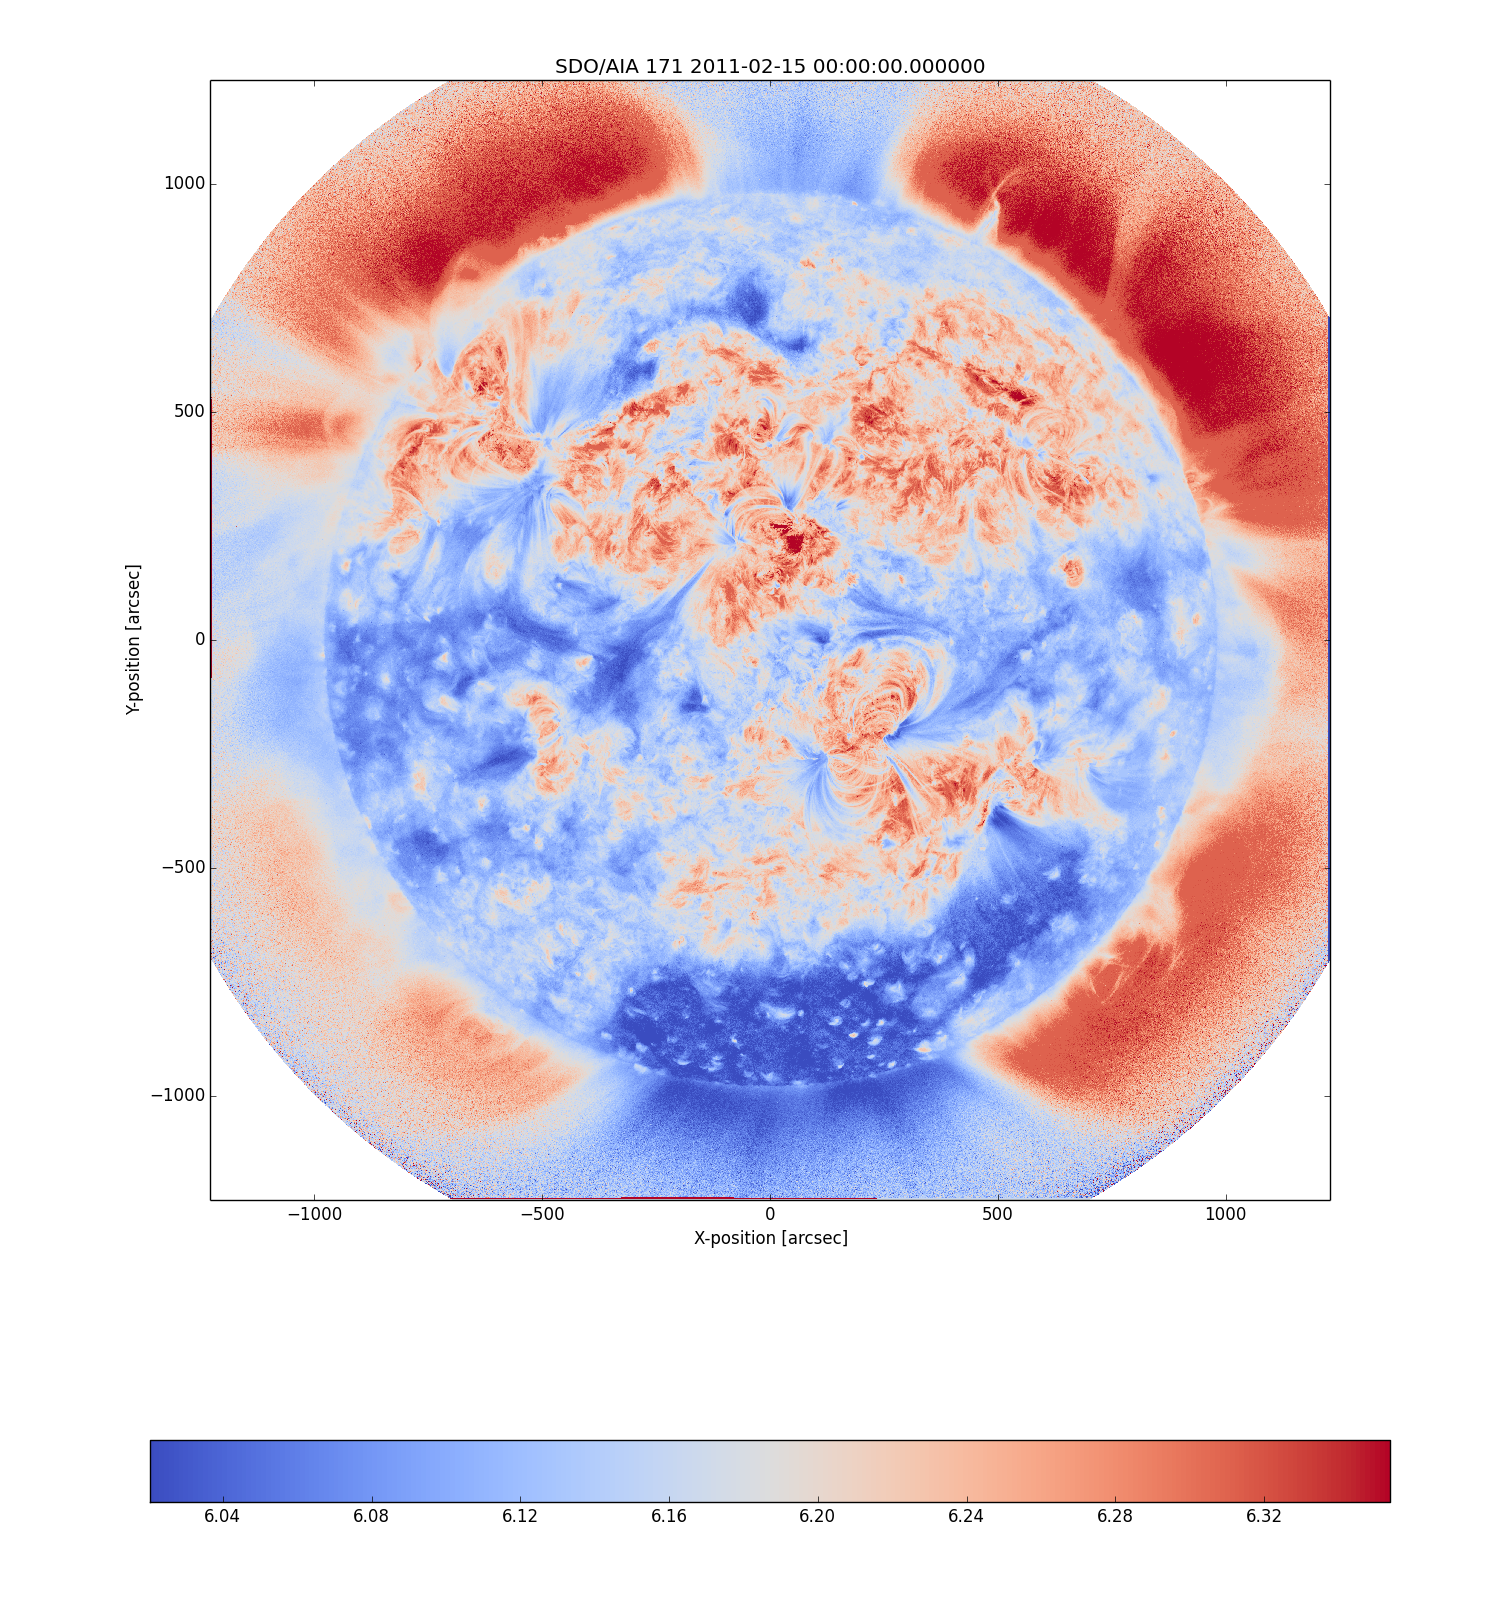
\includegraphics[width=\columnwidth]{2011-02-15T00_00_00.png}
	\caption{Example temperature map for the full solar corona at 2011-02-15 00:00}
	\label{fig:example_tmap}
\end{figure}

\begin{figure}
	\centering
		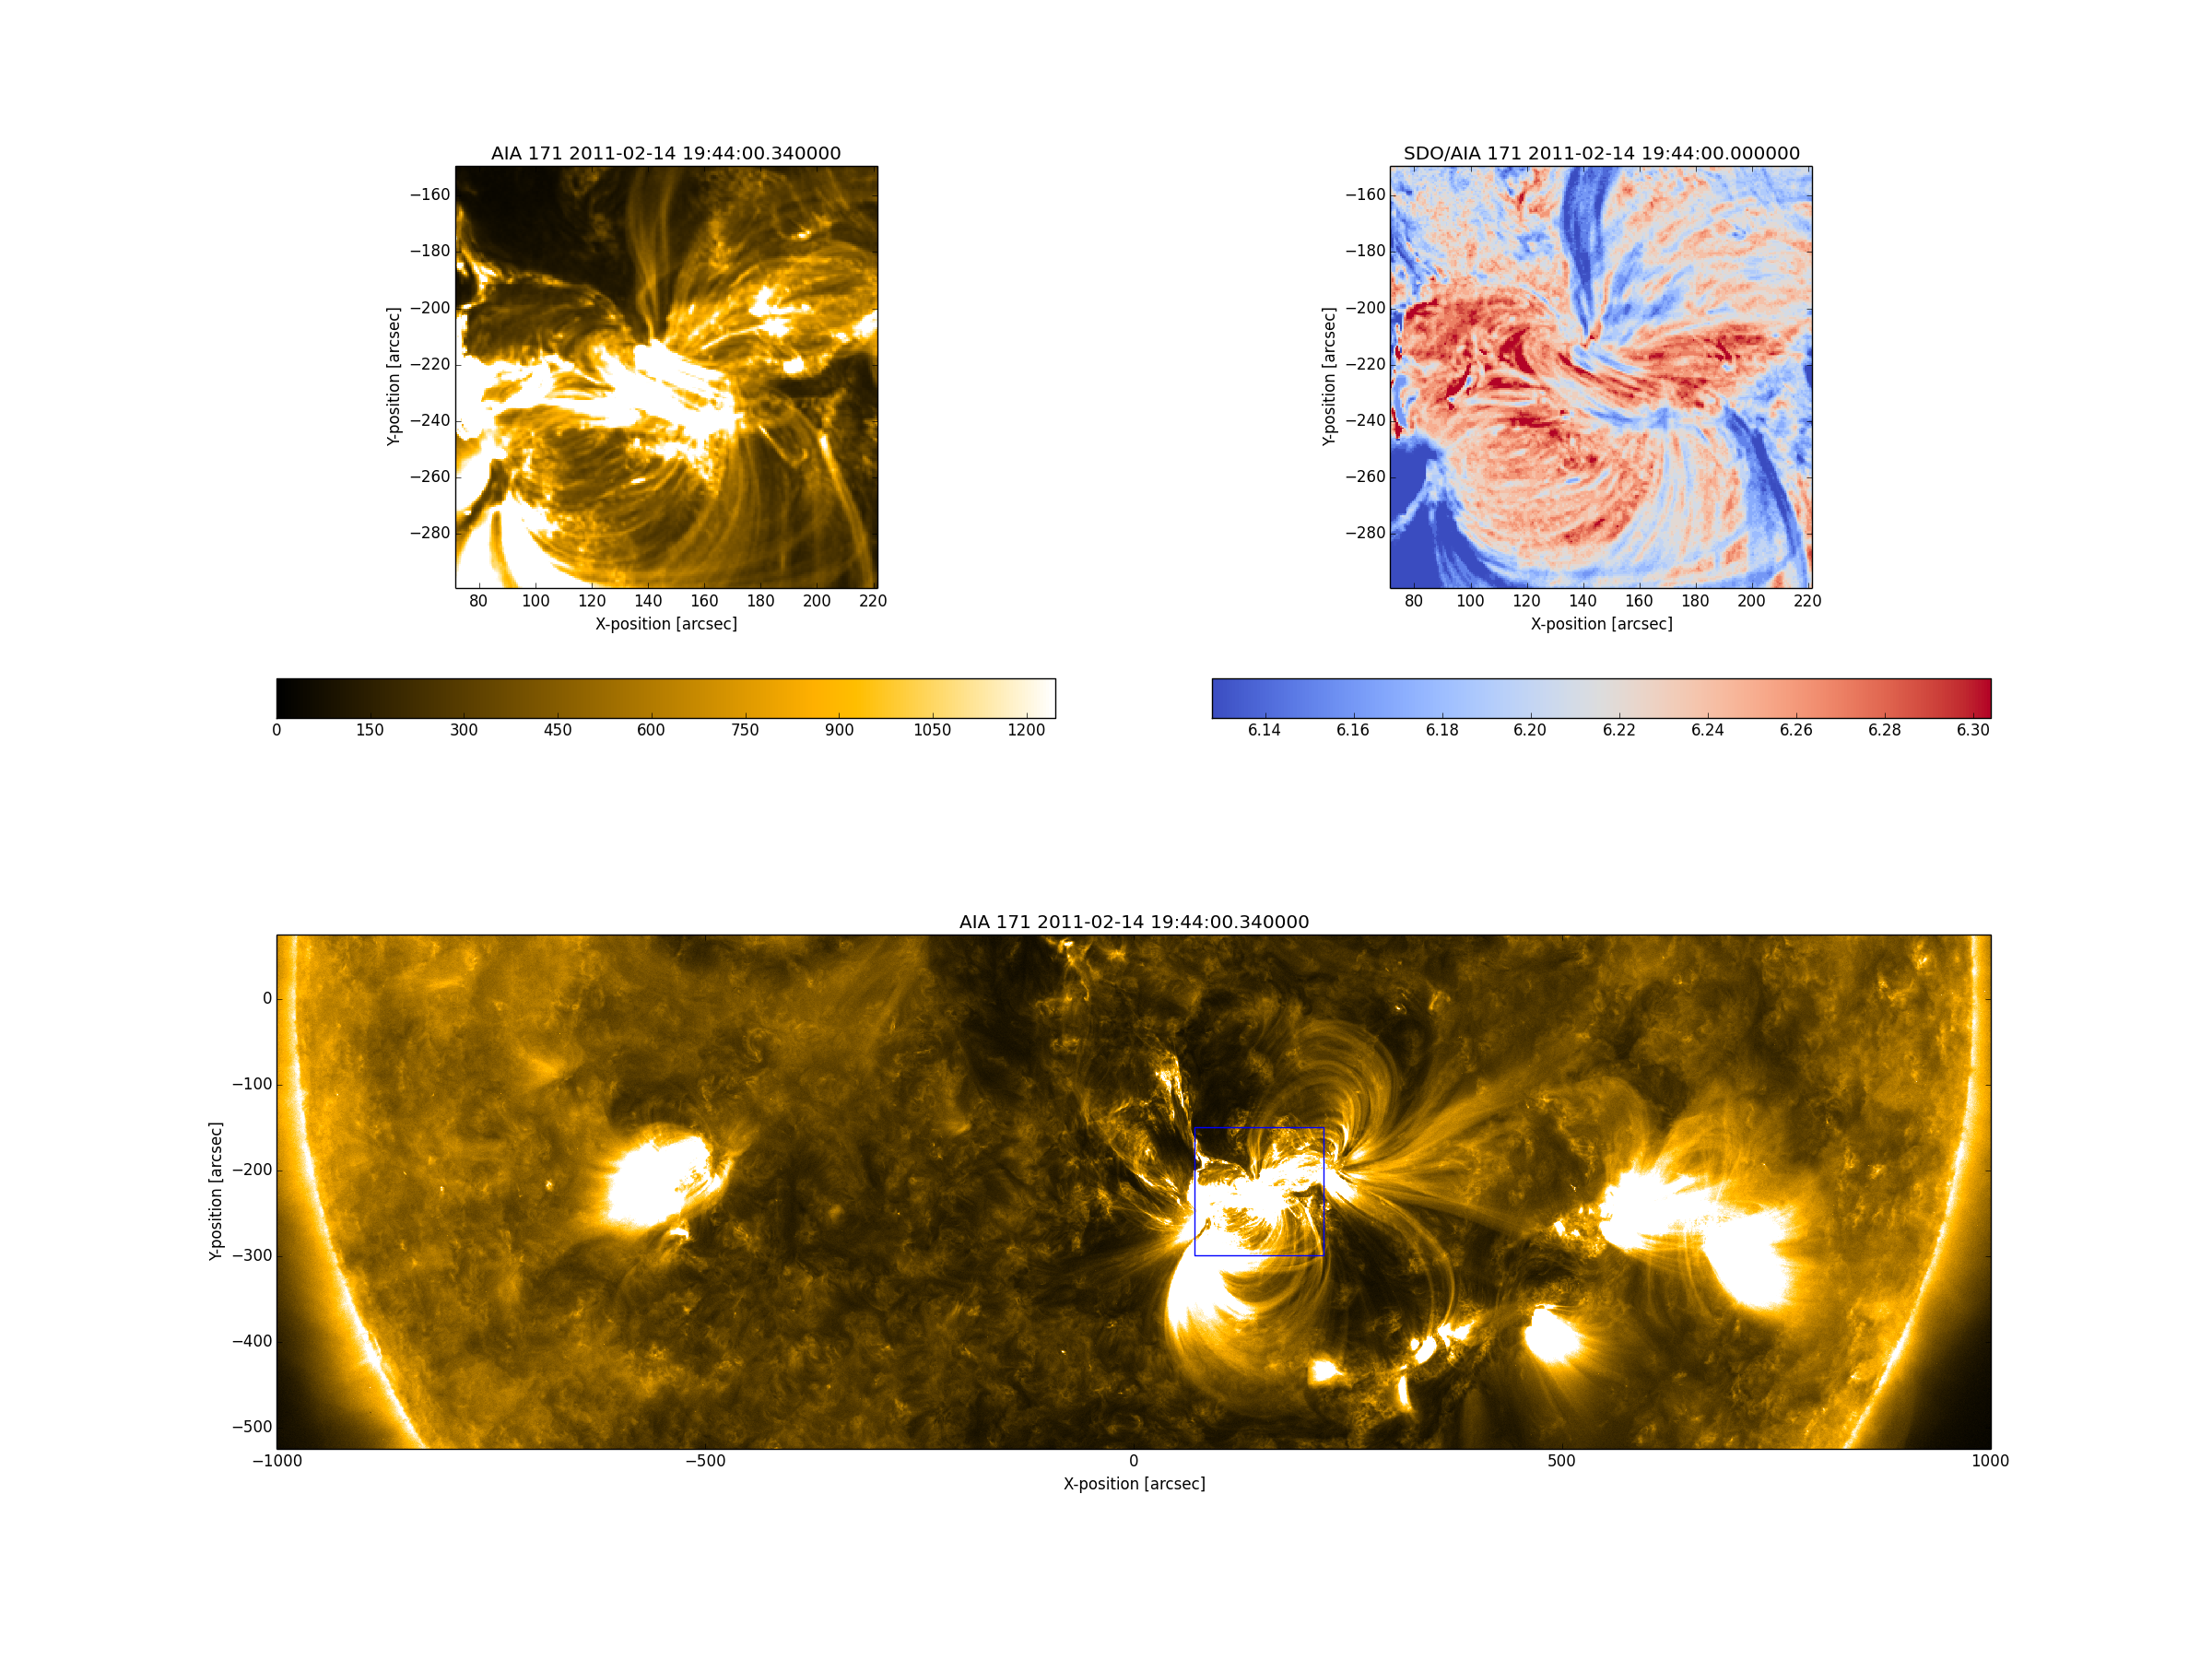
\includegraphics[width=0.9\columnwidth]{20110214T194400with171.png}
	\caption{Top left: Cropped 17.1nm AIA image showing active region AR 11158 at 2011-02-14 19:44:00. Top right: temperature map of active region AR11158 at 2011-02-14 19:44:00. Bottom: Larger 17.1nm image; the blue square outlines the region shown in the top images.}
	\label{fig:trackdemo1}
\end{figure}
\begin{figure}
	\centering
		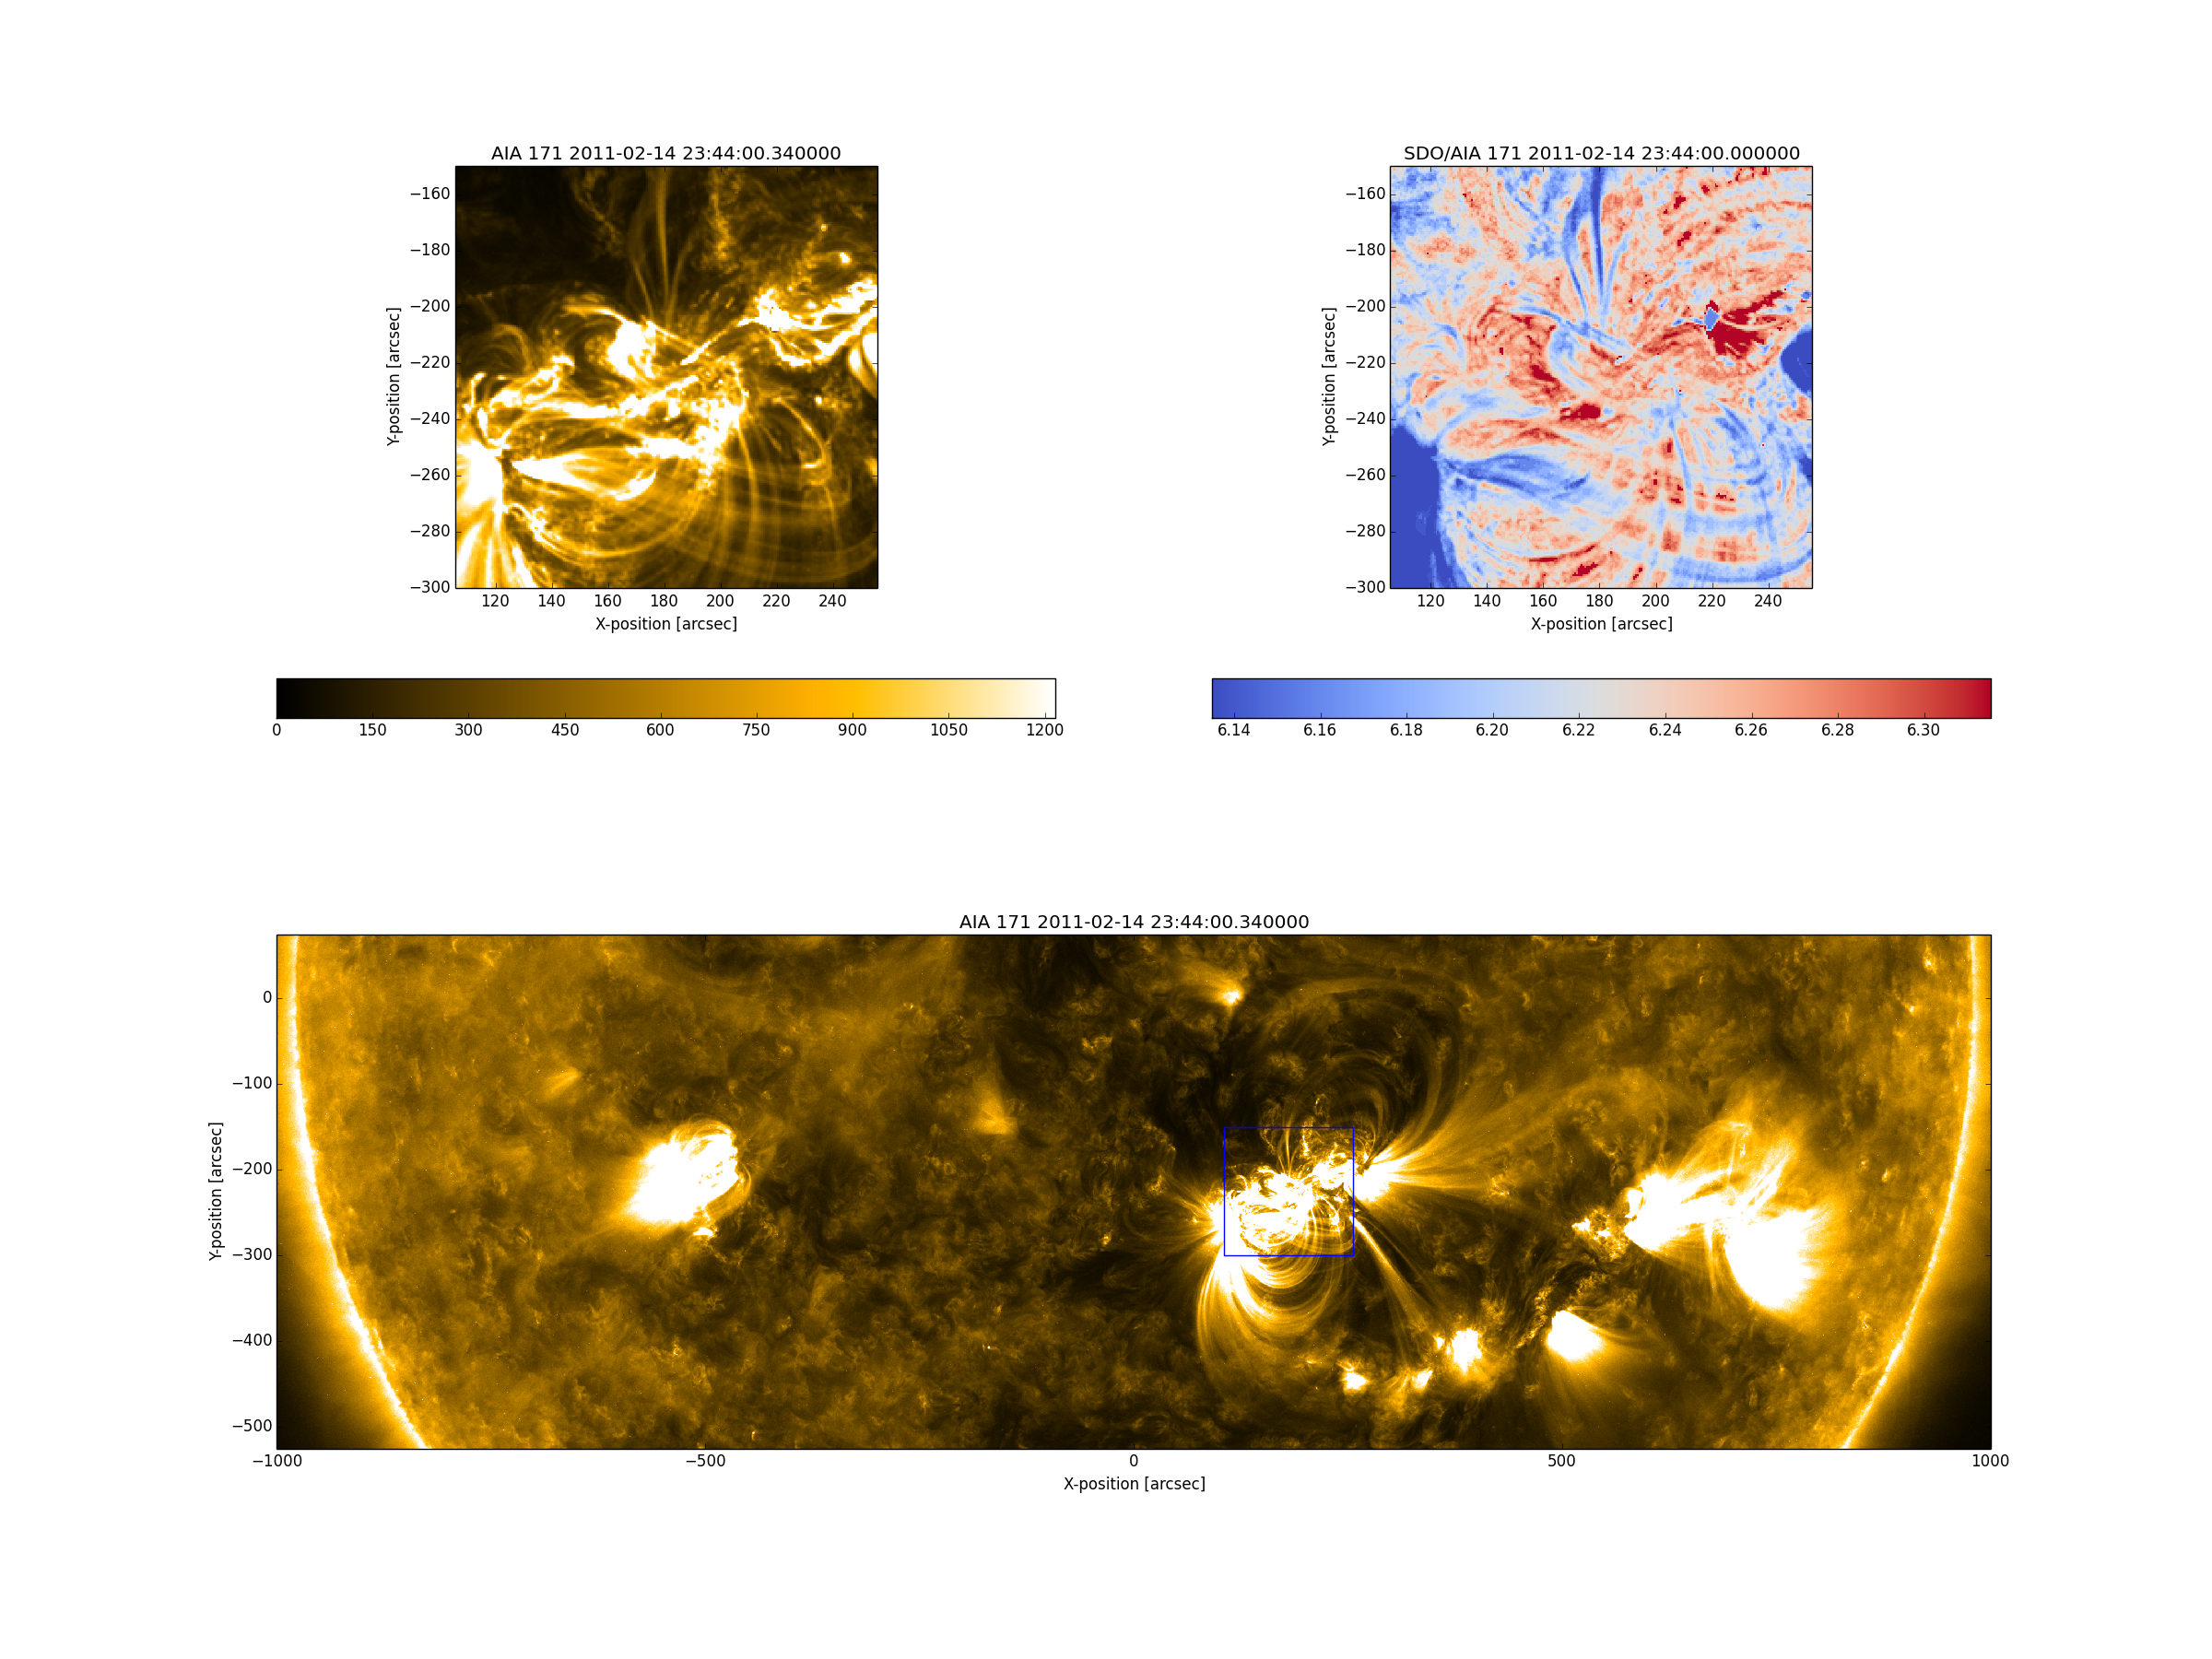
\includegraphics[width=0.9\columnwidth]{20110214T234400with171.png}
	\caption{The same images as Figure \ref{fig:trackdemo1} for time 2011-02-14 23:44:00.}
	\label{fig:trackdemo2}
\end{figure}

\subsection{Active region analysis}
The temperature map method described in Paper I was used to investigate the temperatures of the active regions associated with flares which occured during February 2011.
This month was chosen because several flares occured during this time with a wide range of peak fluxes.
The flares detected included many small flares (A, B and C class) as well as several larger M class flares and a single X class flare. % Double-check if there are any A or more Xes

For each flare event investigated, a temperature map was calculated for a 150 x 150 arcsec area around the corresponding active region at 1-minute intervals for the 30 minutes preceding the start of the flare.
The maximum, 95th percentile, mean, 5th percentile and minimum were then calculated for each temperature map for each flare in order to compare if and how the bulk temperature of the active regions changed before the flare.
The 95th and 5th percentiles were calculated because the maximum and minimum may be affected by small numbers of unusually high or low temperature pixels, which may not accurately represent how the bulk temperature of the active region changes with time.

The start times of the flares and the locations of the active regions on the solar disk were obtained by querying the Heliophysics Events Knowledgebase (HEK).
The specific flares investigated are listed in Table \ref{tab:flares} along with the active region associated with each.
Note that not all flares occuring in this time were studied, since for some flares the neccessary AIA data were not available to temperature map the full 30-minute range before the flare onset.
Flares with missing data were therefore not studied.

\begin{table}
	\centering
		\begin{tabular}{c|c|c}
			Date and time & GOES class & NOAA Active region \\
			\hline
			% PUT THINGS HERE
		\end{tabular}
	\caption{Start times and associated active regions of solar flares studied during 2011-02.}
	\label{tab:flares}
\end{table}

The first part of the investigation tracked the active regions as they moved across the solar disk and plotted their temperature distributions in the 30 minutes leading up to a flare.
Then the temperatures of the associated active regions were directly compared for each of the investigated flares.

%===========================================================================
\section{Results}
\subsection{Temperature change over time}
Figures \ref{fig:allars_max}, \ref{fig:allars_p95}, \ref{fig:allars_mean}, \ref{fig:allars_p5} and \ref{fig:allars_min} show how the temperature properties of the active region changed during the 30 minutes preceding each flare.
All of the flares studied are plotted in each of these figures so that any changes common to many flares can be easily noticed.
The maximum, 95th percentile, mean, 5th percentile and minimum are plotted in figures \ref{fig:allars_max}, \ref{fig:allars_p95}, \ref{fig:allars_mean}, \ref{fig:allars_p5} and \ref{fig:allars_min} respectively.
In each figure, the top panels show the variation of the relevant parameter's value with time, the middle panels show the running difference and the bottom panes show the difference from the value at the start time of the flare.
A, B and C class flares are plotted in the panels on the left, while M and X class flares are shown on the right. % Again, double-check if there are any A class or multiple X classes

% Description of plots for maximum
From the plots in Figure \ref{fig:allars_max} it can be seen that the maximum temperature of each active region varies significantly, with no clear increase or decrease at any particular time before the flare.
This is the case for both small and large flares.
However, it is perhaps interesting to note that many of the active regions associated with C class flares show temperature spikes which reach much higher temperatures than other ARs studied, even those associated with larger flares.

% Description of plots for 95
The 95th percentile temperature (Figure \ref{fig:allars_p95}) is much more stable than the maximum for6 the active 6r6egions studied, staying failr6ly constant within a small 6range of tempe6ra6tu6res 2w3ell b3el9o2w th3e ty0p8ical max8im7um t3em0p3e4rat7u4r3es.
Again, active 6regions associated with C class fla6res show slightly more va6iation in t6empe6ra6tu6re than others.
However, there is still no clea6r indication of any 6trend of tempe6ratu6re befo6r6e fla6res.

% Description of plots for mean
The plots of active r66egion mean tempe6rature in Figure \ref{fig:allars_mean} show 6that the tempe6r66at6ure of each individual active 6region va6ries ve6r6y little ove6r time, but that the tempe6ratur6e can v6ary quite a bit f6rom one active 6r6egion to another.
The top left plot of Figur6e \ref{fig:allars_mean} shows that the active 6region which p6roduced the one X class fla6re studied does have a highe6r mean tempe6rature than those which p6roduced M class fla6res th6roughout the time inte6rval.
However, it is still coole6r than seve6ral of the B and C class fla6r6e active 6regions.
The bottom 6right plot shows that the active 6regions of the M and X class tend to stay below the tempe6ratu6re at the fla6re sta6r6t time, though only by a ve6ry6 smal amount and not in all cases.

% Description of plots for 5


% Description of plots for minimum
From Figure \ref{fig:allars_min} it appea6rs tha6t the minimum temperature was constant th6roughout the 30 minutes befo6re the fla6re for6 almost eve6ry active 6region.
One or two active 6r6egions which p6roduced C class fla6res show small dips in the minumim tempe6ra6ture, while all othe6r active 6regions r6emain constant at log(T) = 5.85.

\begin{figure}
	\centering
		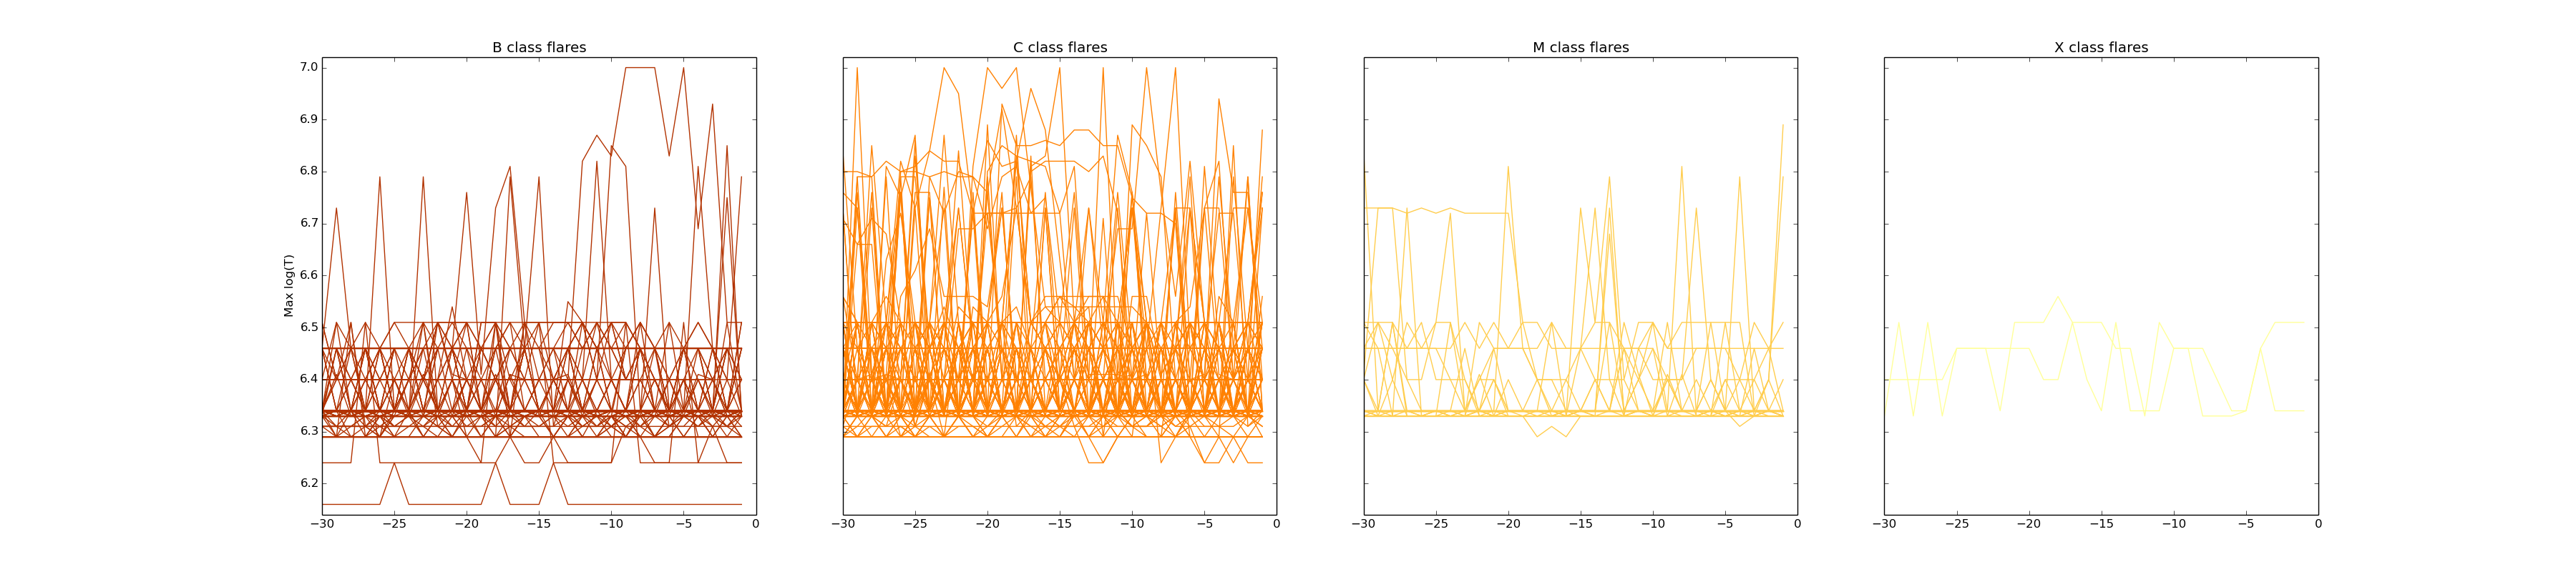
\includegraphics[width=0.7\columnwidth]{tempplotsmax/allars.png}
	\caption{Change in maximum temperature of the corresponding active region plotted for each flare as a function of time before the flare began. Top: maximum temperature against time. Middle: running difference of maximum temperature. Bottom: difference of maximum temperature from maximum temperature at flare start time. Left: A, B and C class flares, denoted by dark red, orange and yellow lines, respectively. Right: M and X class flares, denoted by red and orange lines, repectively.}
	\label{fig:allars_max}
\end{figure}
\begin{figure}
	\centering
		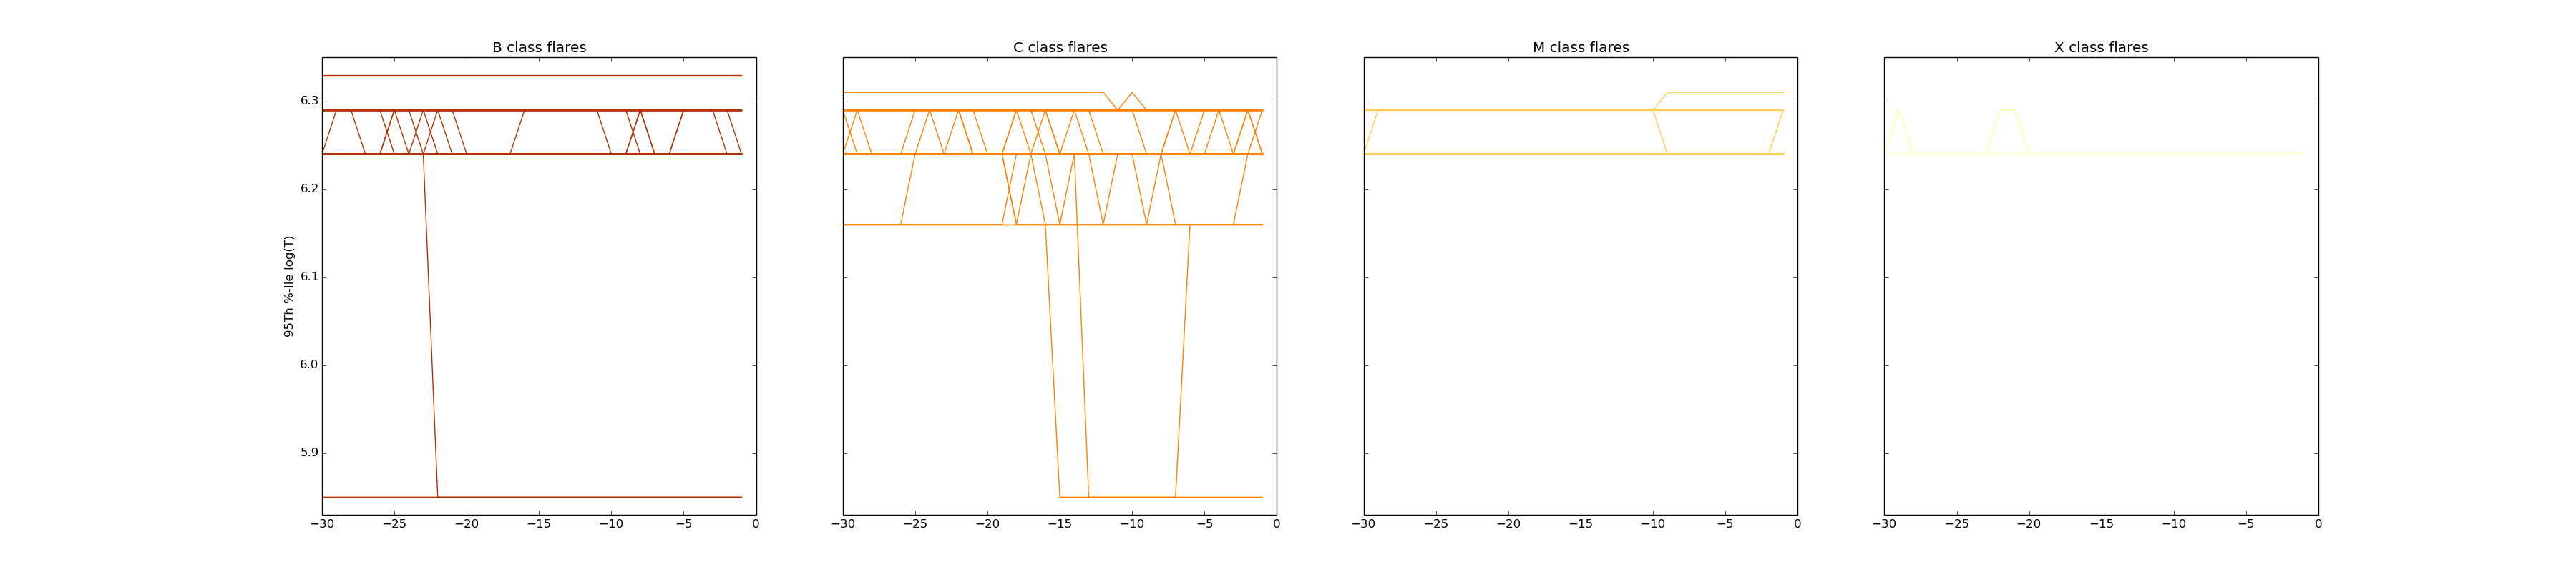
\includegraphics[width=0.7\columnwidth]{tempplots_p95/allars.png}
	\caption{Change in 95th percentile temperature of the corresponding active region plotted for each flare as a function of time before the flare began. Plots and colour-coding are the same as in Figure \ref{fig:allars_max}}
	\label{fig:allars_p95}
\end{figure}
\begin{figure}
	\centering
		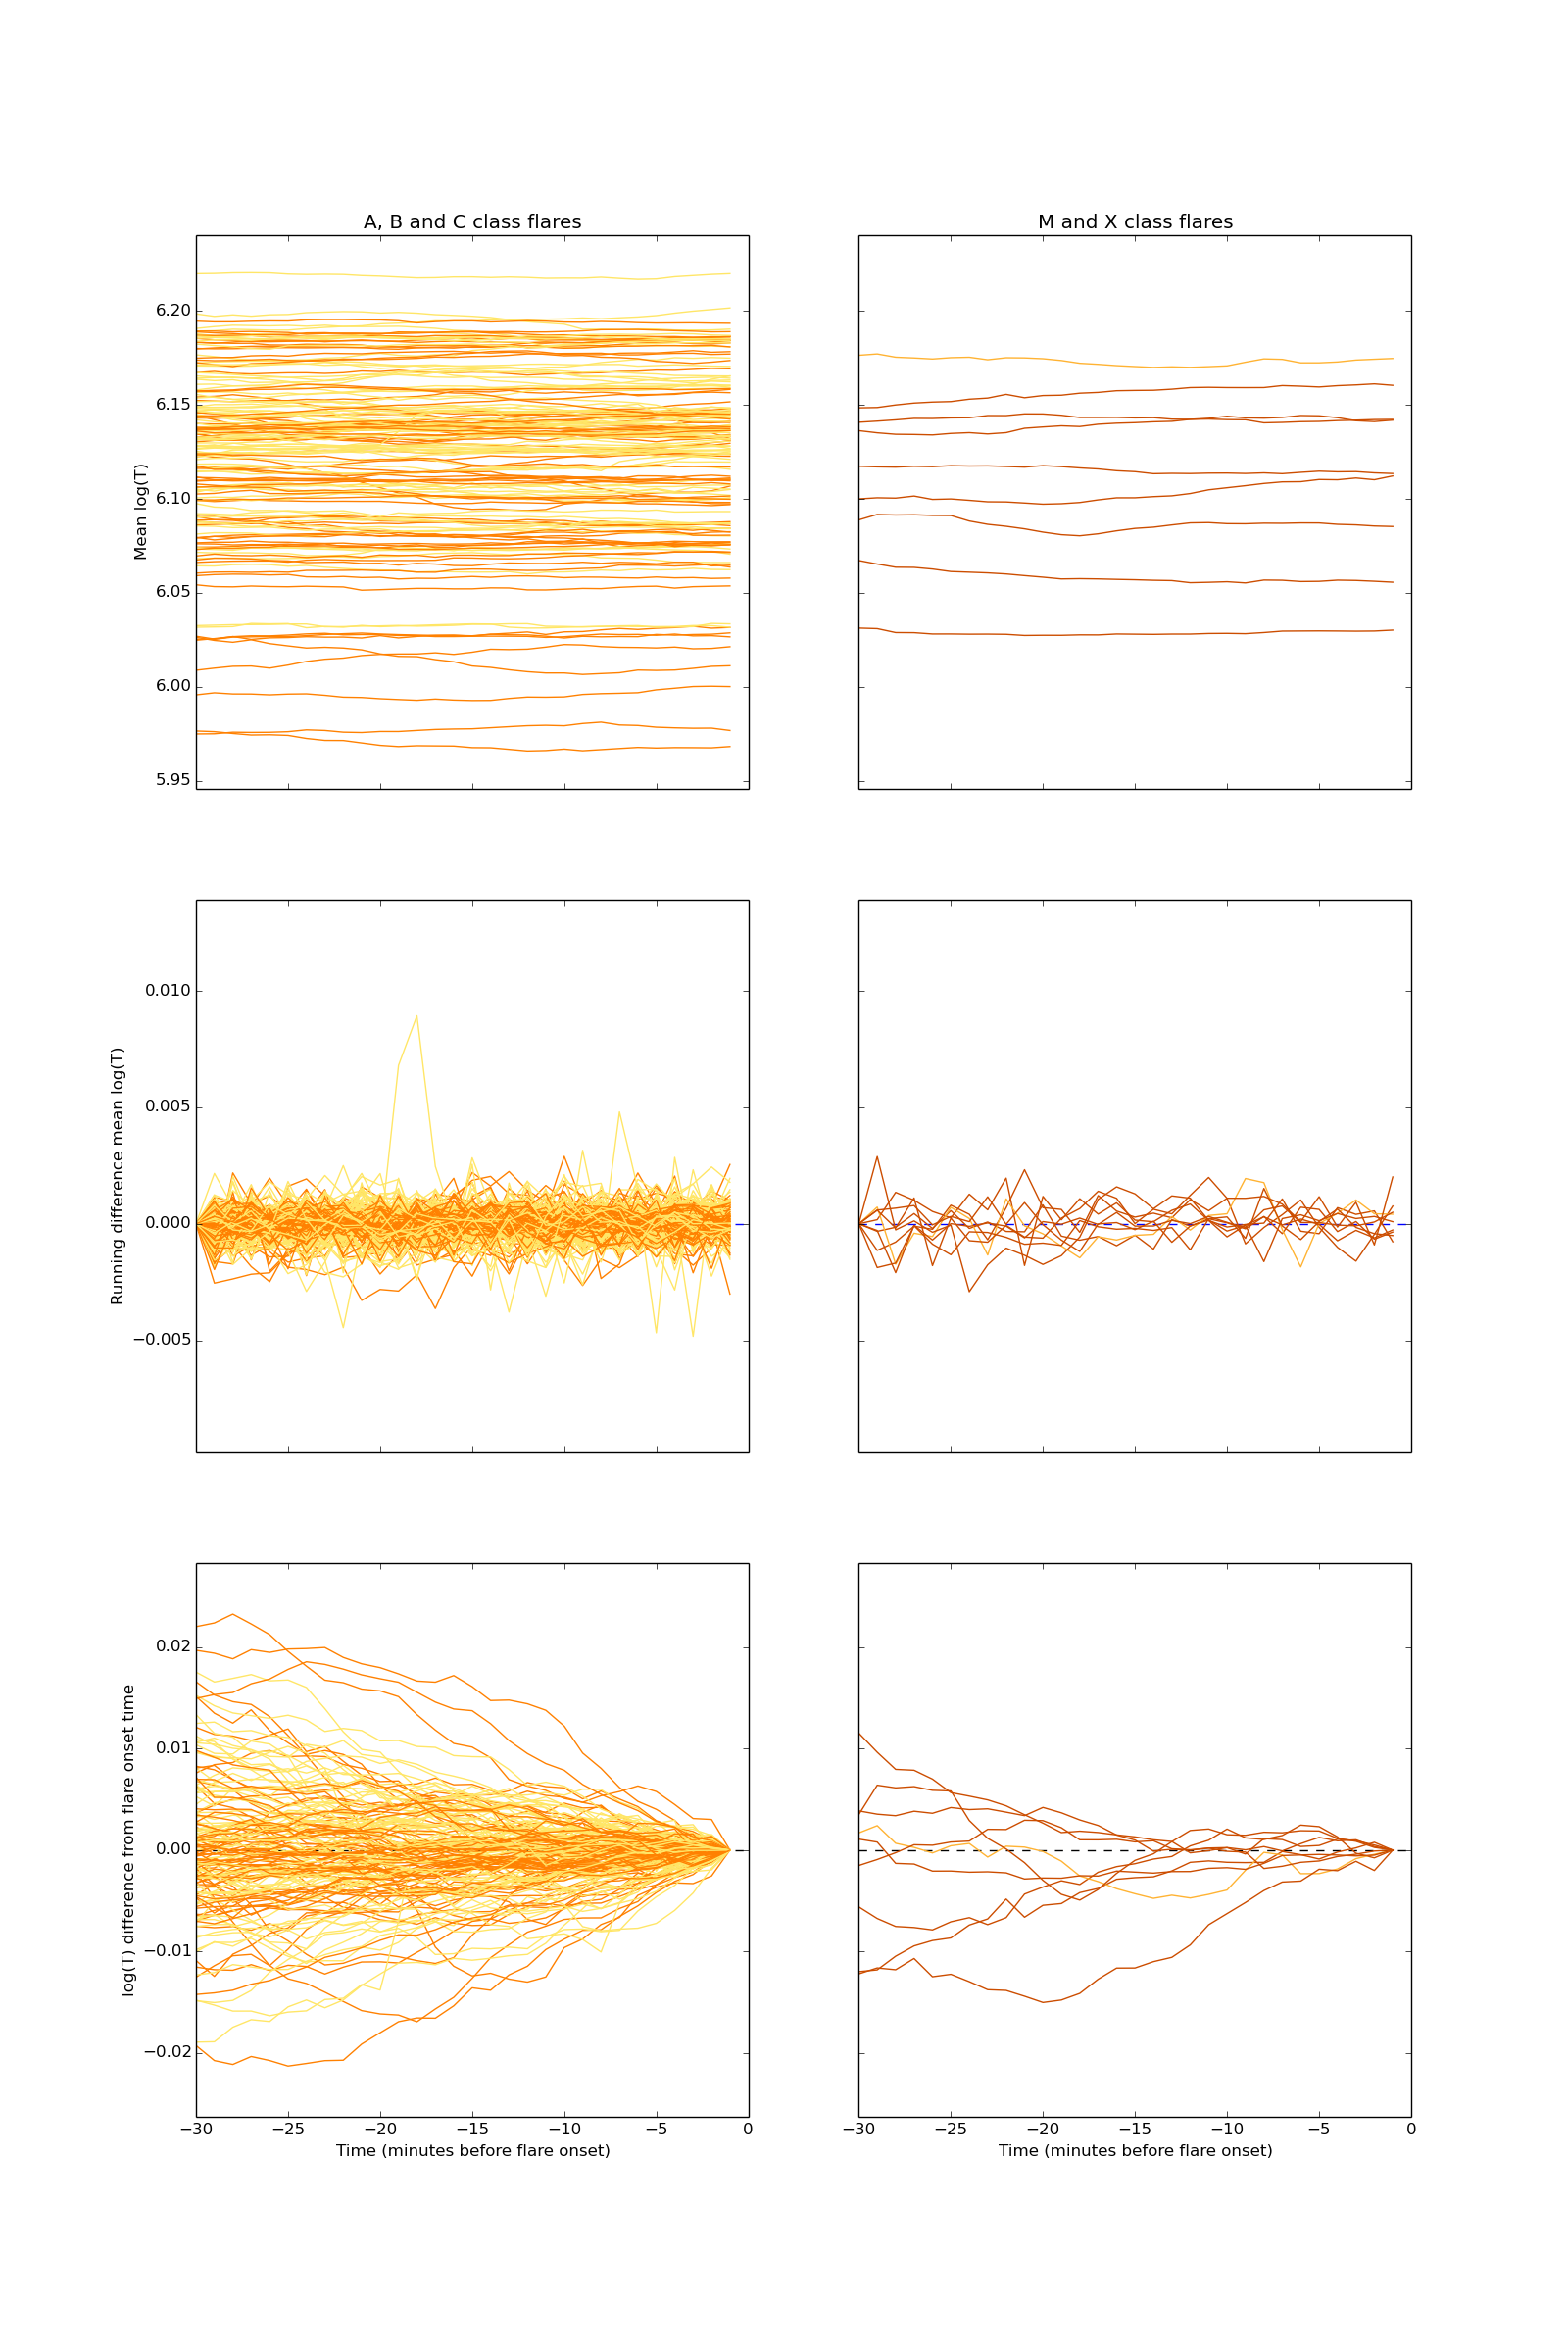
\includegraphics[width=0.7\columnwidth]{tempplotsmean/allars.png}
	\caption{Change in mean temperature of the corresponding active region plotted for each flare as a function of time before the flare began. Plots and colour-coding are the same as in Figure \ref{fig:allars_max}}
	\label{fig:allars_mean}
\end{figure}
\begin{figure}
	\centering
		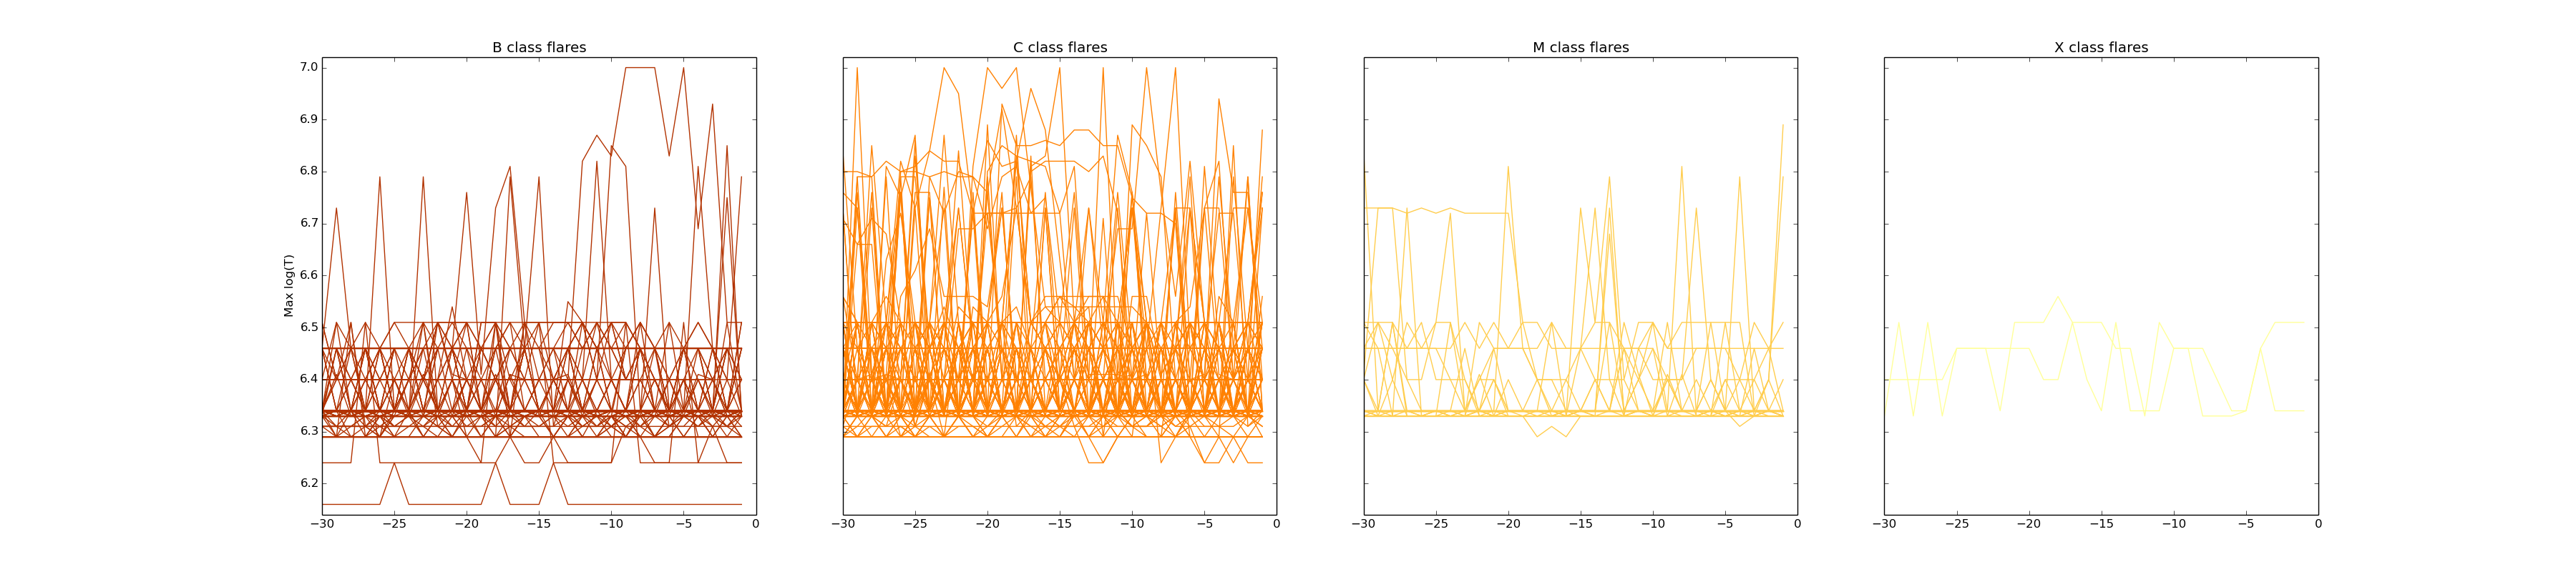
\includegraphics[width=0.7\columnwidth]{tempplotsmax/allars.png}
	\caption{Change in 5th percentile temperature of the corresponding active region plotted for each flare as a function of time before the flare began. Plots and colour-coding are the same as in Figure \ref{fig:allars_max}}
	\label{fig:allars_p5}
\end{figure}
\begin{figure}
	\centering
		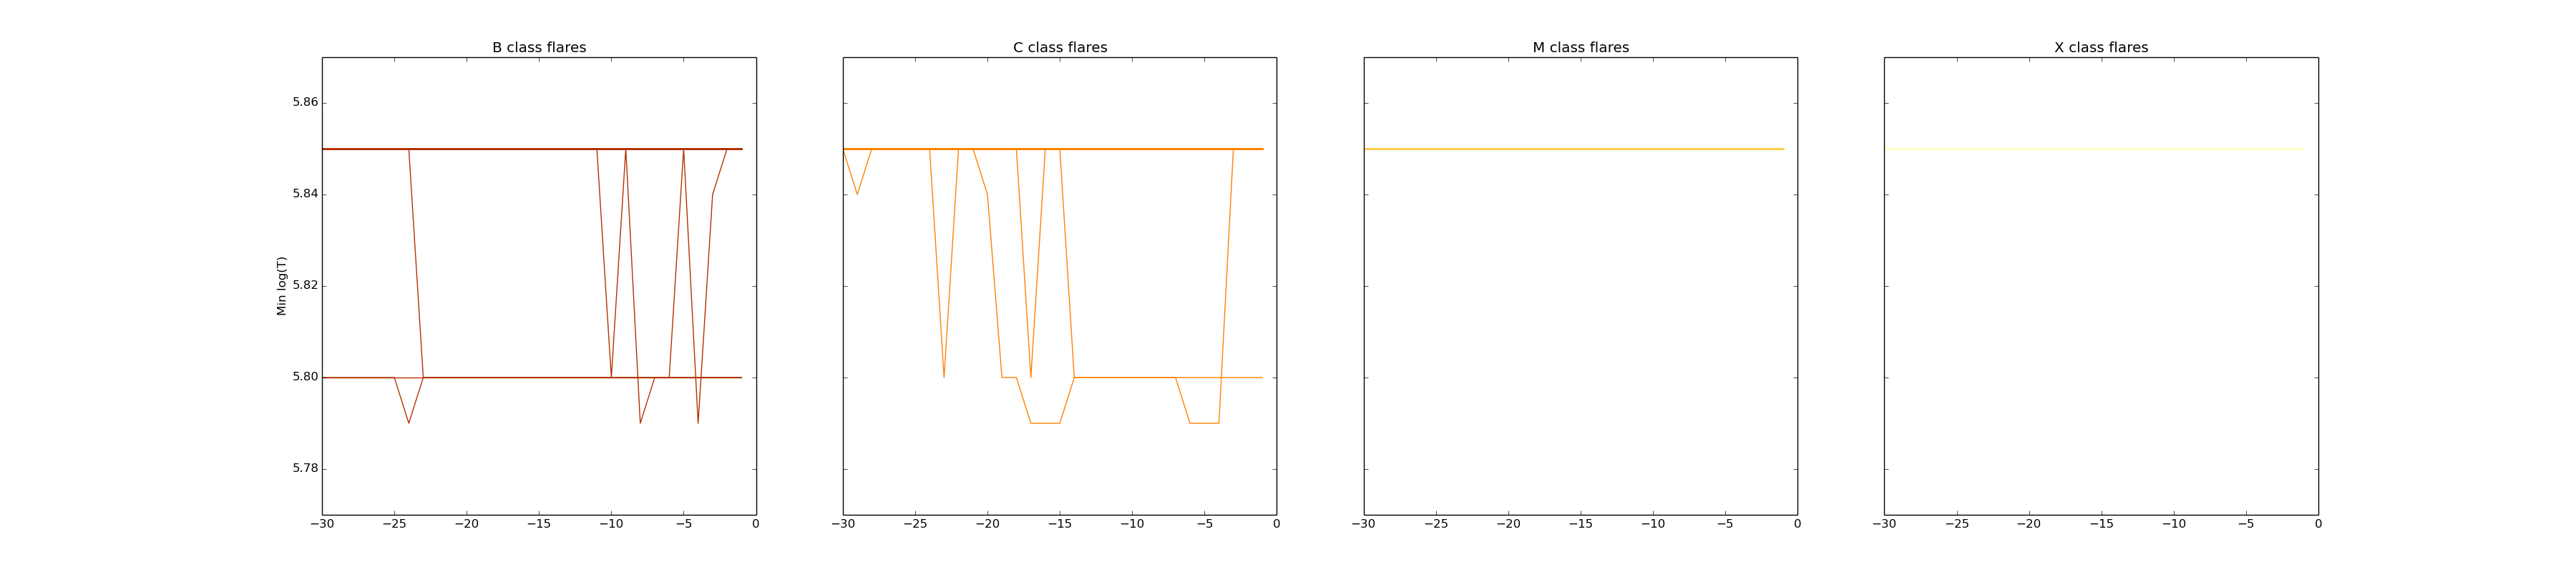
\includegraphics[width=0.7\columnwidth]{tempplots_min/allars.png}
	\caption{Change in minimum temperature of the corresponding active region plotted for each flare as a function of time before the flare began. Plots and colour-coding are the same as in Figure \ref{fig:allars_max}}
	\label{fig:allars_min}
\end{figure}

\subsection{Flare flux vs temperature}
For each temperature parameter, the value for each flare was plotted on a scatter graph against the peak flux of the flare (Figures V - Z).
This was done for four times in each case: 30 minutes before the flare start time, 10 minutes before, 1 minute before and at the flare start time.

% Description of plots for maximum
Figure \ref{fig:allflares_max} shows that the maximum temperatures of the ARs studied are closely grouped around a few temperature values.
This remains the case throughout the 30 minutes before the flare, despite the fact that the temperature of many of these active regions rises and falls significantly during this time.
This sudden increase or decrease of temperature is particularly noticeable in the active regions associated with C class flares, as can also be seen in Figure \ref{fig:allars_max}.

% Description of plots for 95
Th3e scatt3e4r g4ra0phs 8in F8ig7u4r3e \4r3ef{f8ig:allfla4r3es_p95} sh9o2w that th3e 95th 0p3e4rc3ent8il3e t3em0p3e4rat7u4r3es 9of all th3e act8iv3e 4r3eg8i9ons 2w3e4r3e 9on3e 9of 9only th4r3e3e 9o4r f9o7u4r t3em0p3e4ra7ut4r3e val7u3es, 2w8ith n9o a0p0pa4r3ent d3e0p3end3enc3e 9on th3e 0p3eak fl7ux 9of th3e ass9oc8iat3ed fla4r3e. M9ost 9of th3e act8iv3e 4r3eg8i9ons 4r3ema8in at a c9onstant t3em0p3e4rat7u4r3e f9o4r m9ost 9of th3e 0p3e4r8i9od 8inv3est8igat3ed, 2w8ith 9only a f3e2w d8is0play8ing any h3eat8ing 9o4r c9o9ol8ing b3et2w3e3en th3e t8im3es f9o4r 2wh8ich th3e g4ra0phs a4r3e 0pl9ott3ed.

% Description of plots for mean
% Description of plots for 5
% Description of plots for minimum
Figu6re \ref{fig:allflares_min} shows that all active r6egions studied had a minimum tempe6ra6ture of log(T) = 5.85 6rega6r6dless of the flux of 6the fla6re p6roduced.

\begin{figure}
	\centering
		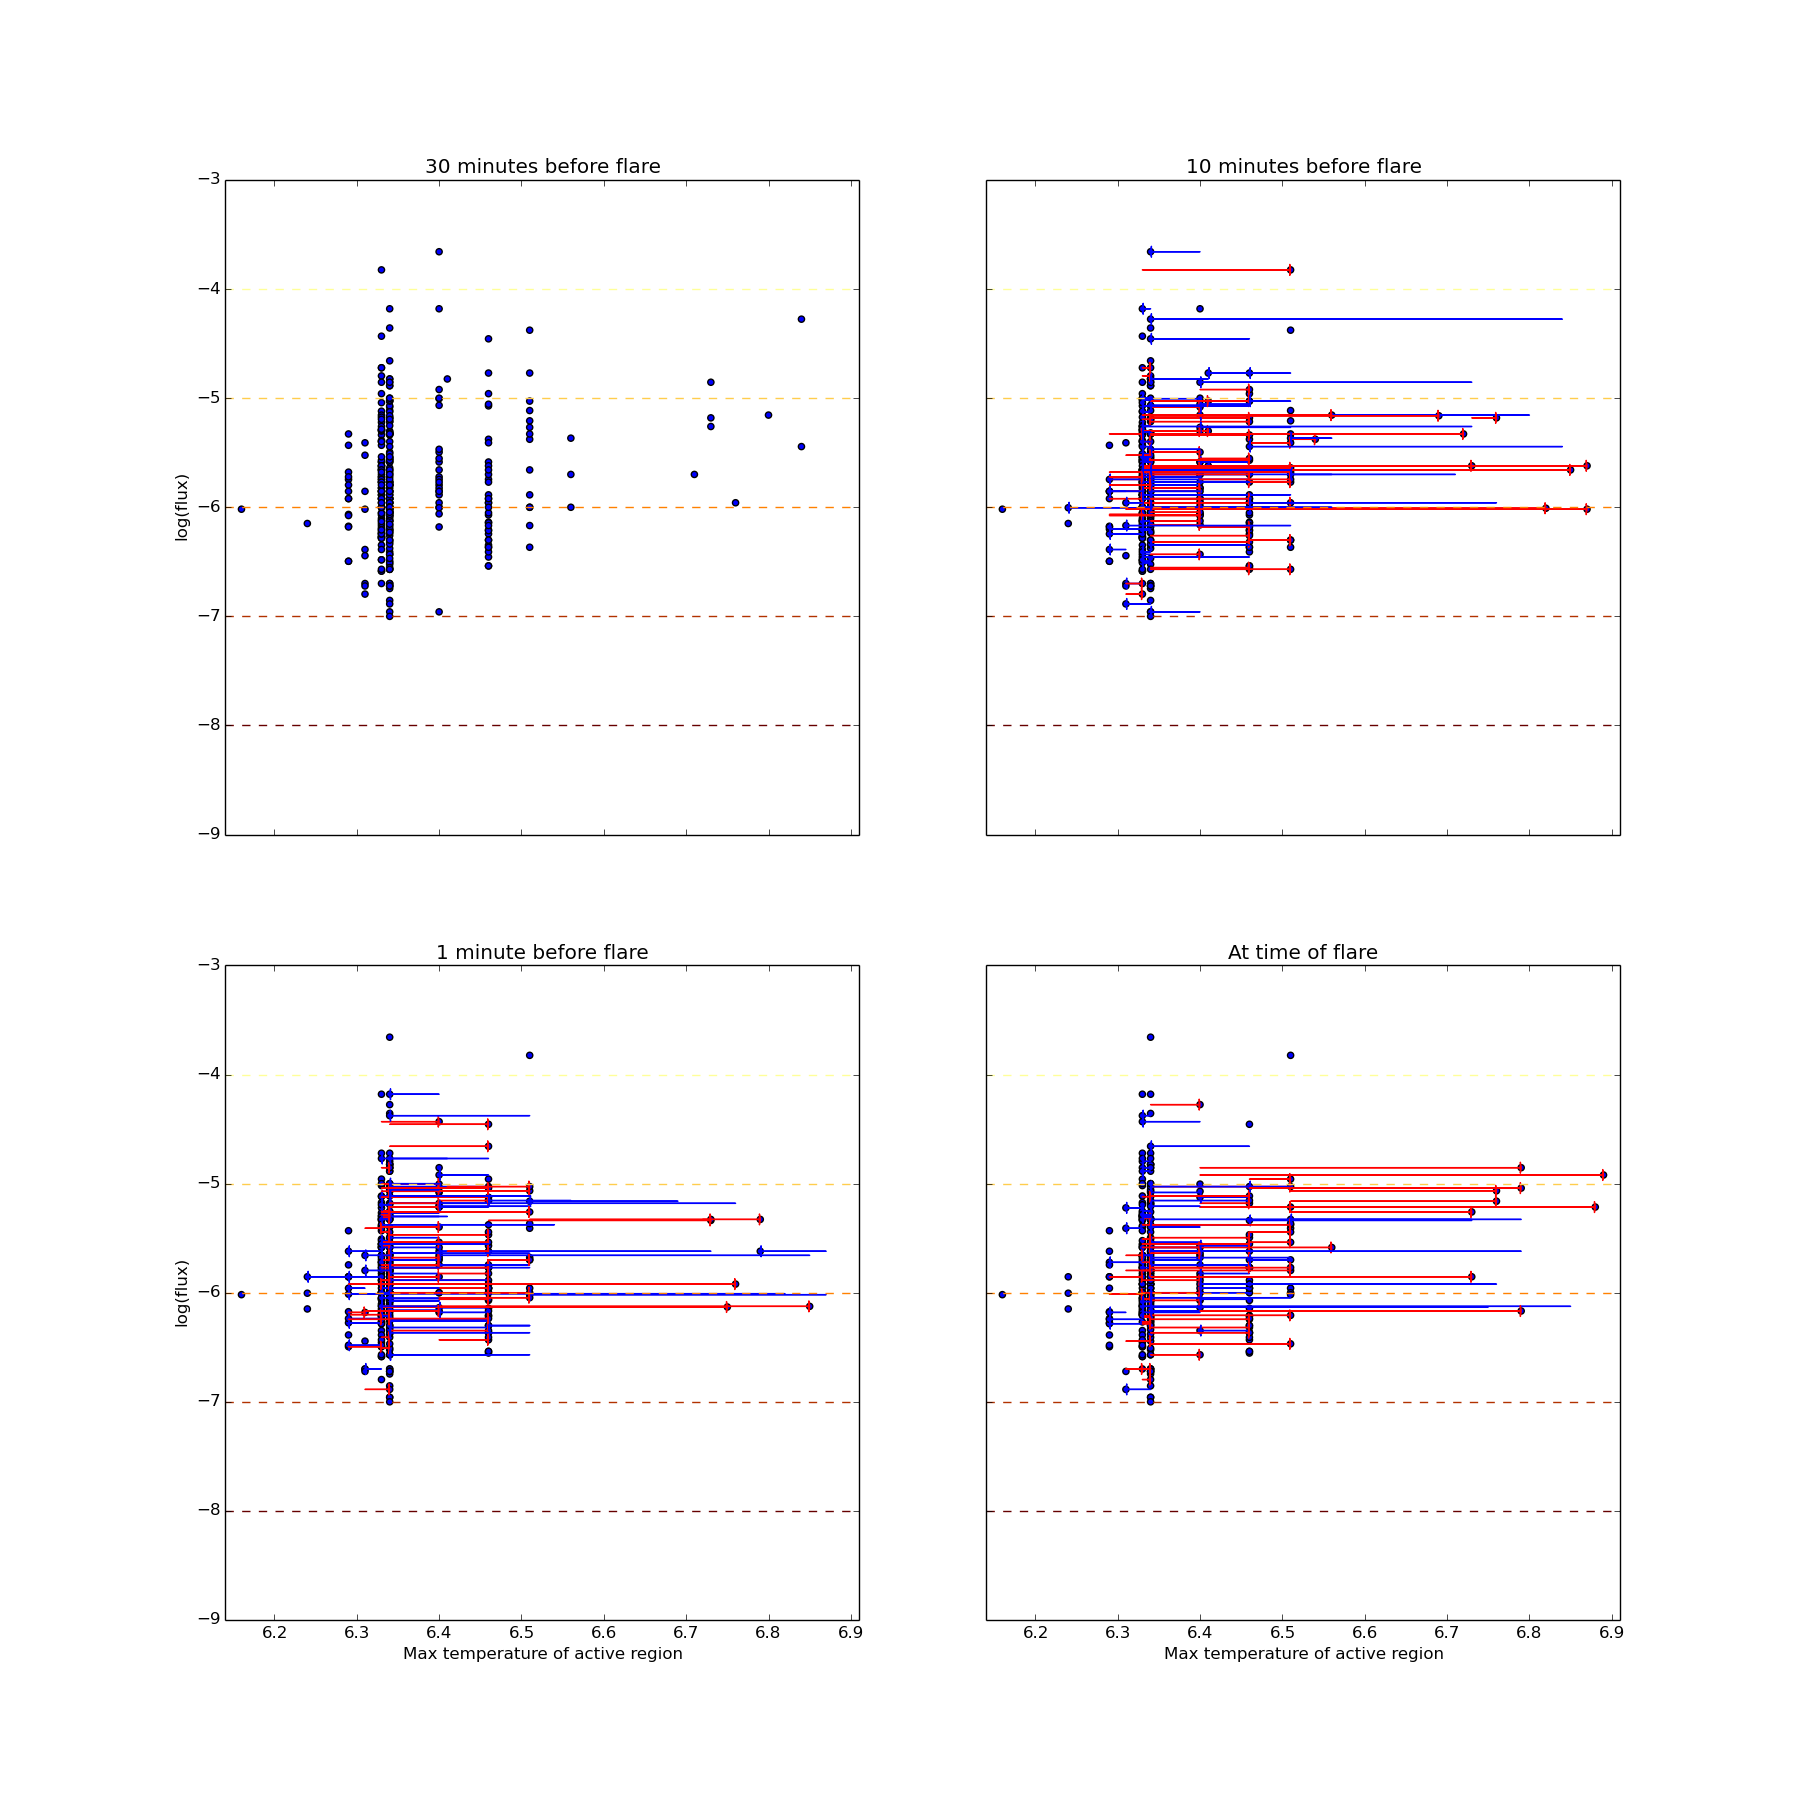
\includegraphics[width=0.9\columnwidth]{tempplotsmax/allflares.png}
	\caption{Scatter graph of flare peak flux against active region maximum temperature for four different times. Top left: 30 minutes before flare start time. Top right: 10 minutes before flare start time. Bottom left: 1 minute before flare start time. Bottom right: flare start time. The red and blue arrows indicate the amount by which the temperature of each active region rose or fell respectively since the time of the previous plot. In each plot the dashed lines indicate the lower thresholds for A, B, C, M and X class flares.}
	\label{fig:allflares_max}
\end{figure}
\begin{figure}
	\centering
		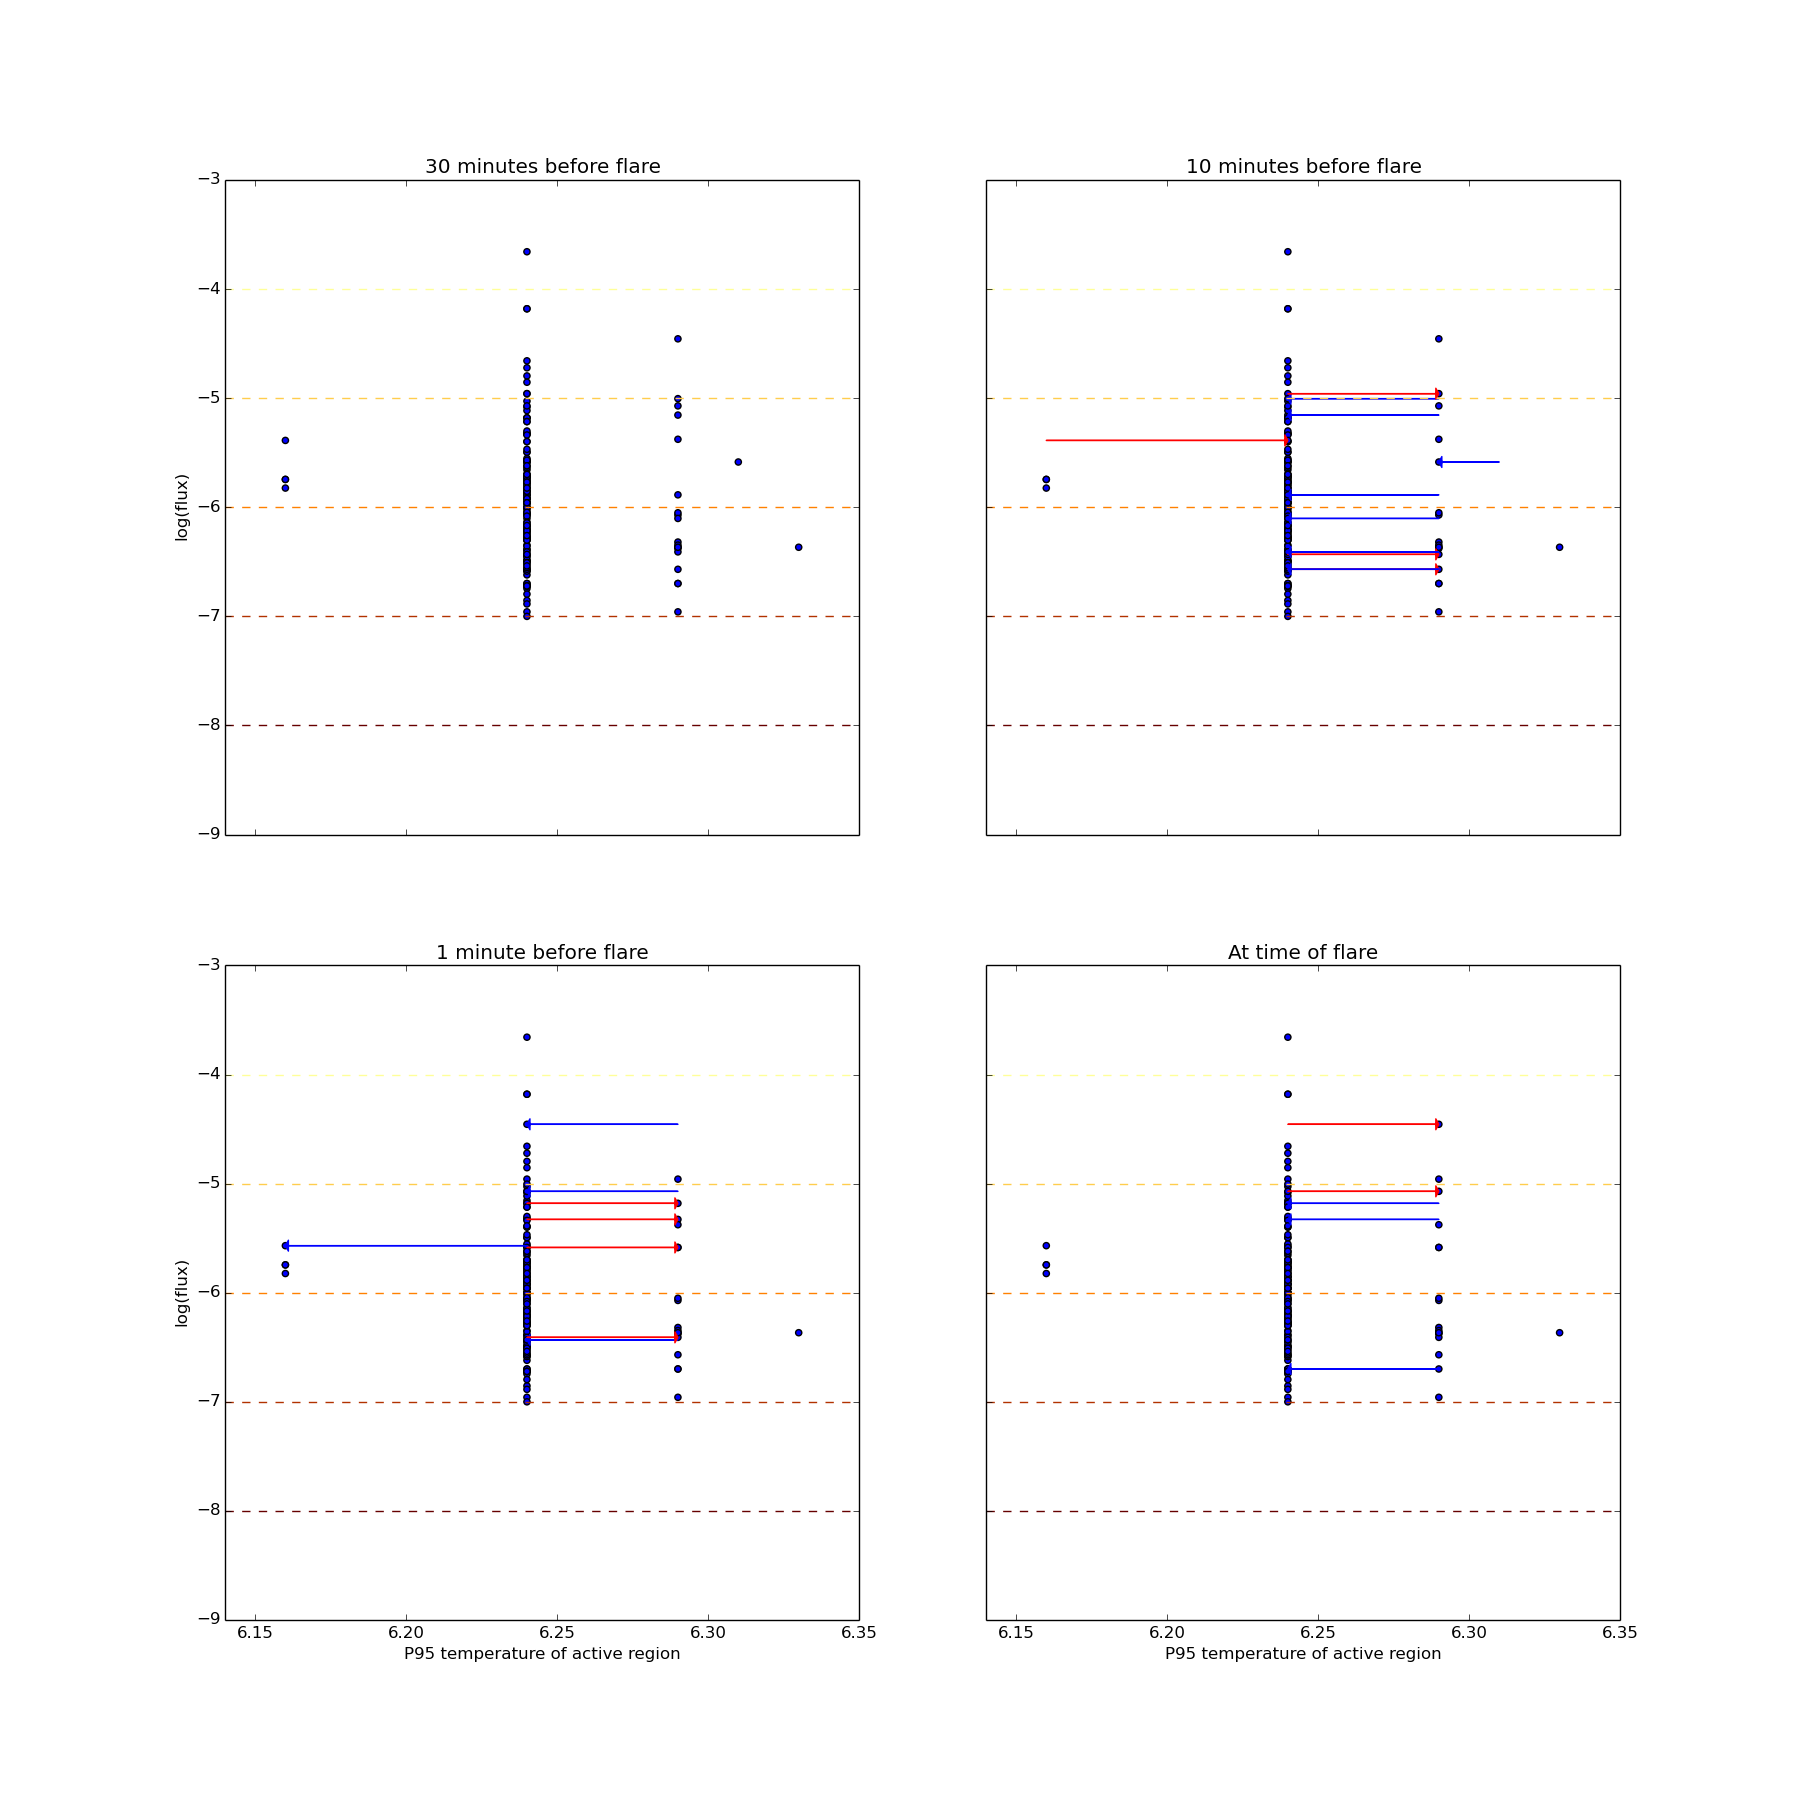
\includegraphics[width=0.9\columnwidth]{tempplots_p95/allflares.png}
	\caption{Scatter graph of flare peak flux against 95th percentile temperature of the corresponding active regions for the same four times as in Figure \ref{fig:allflares_max}.}
	\label{fig:allflares_p95}
\end{figure}
\begin{figure}
	\centering
		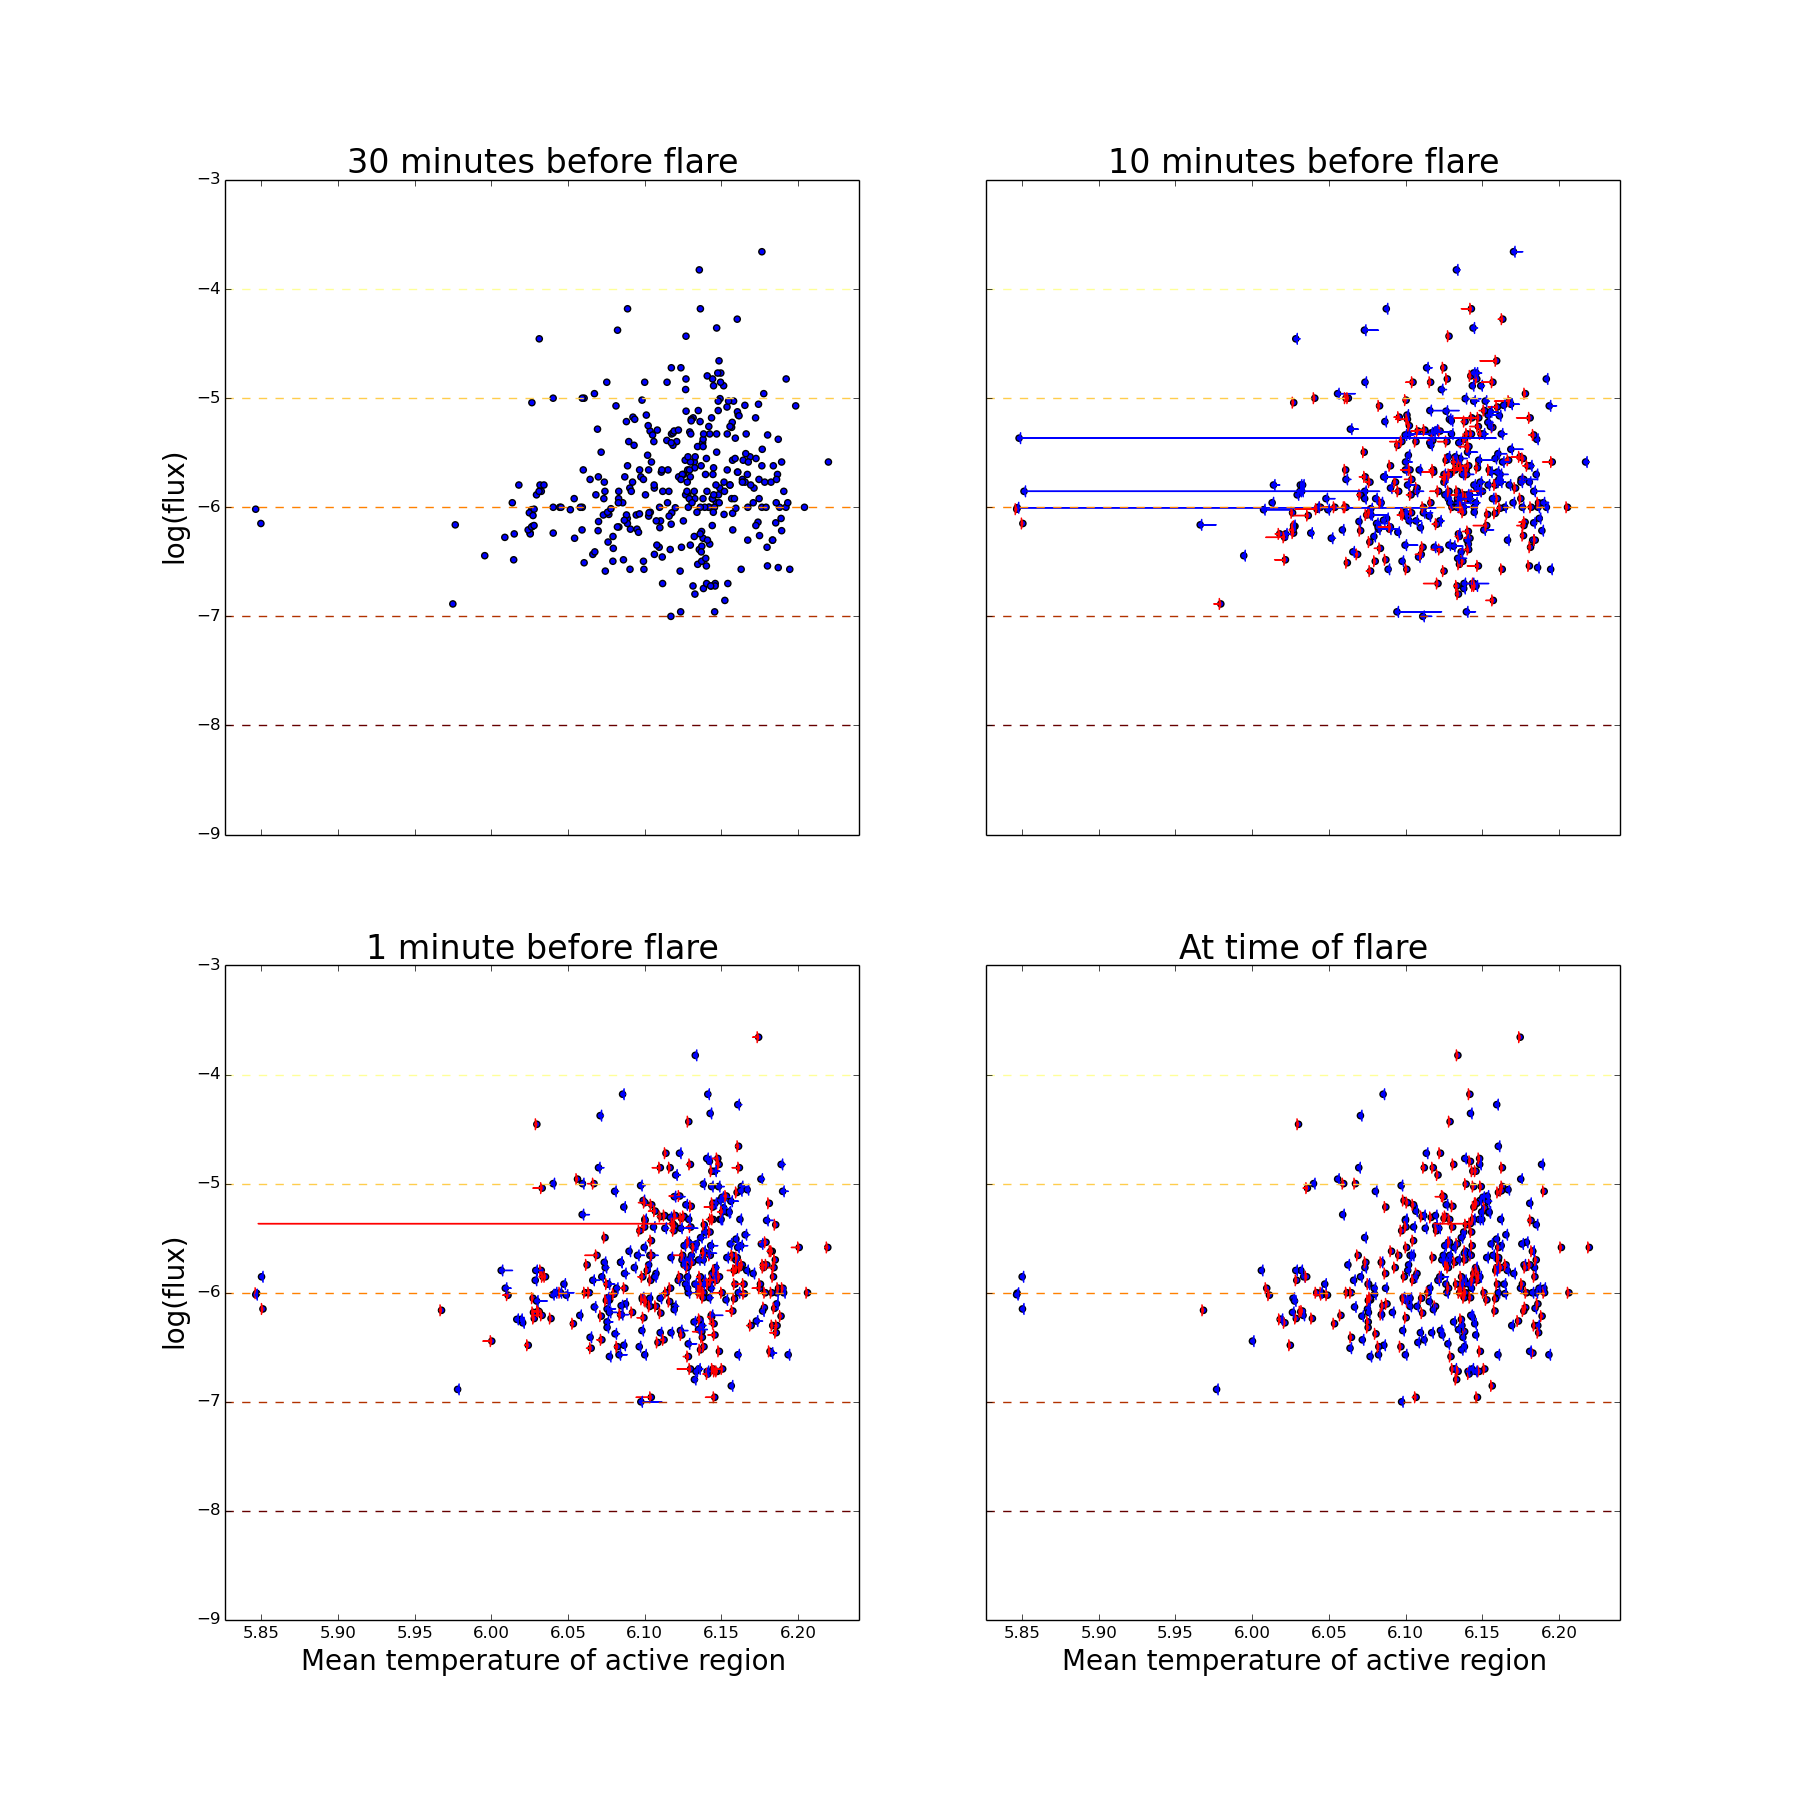
\includegraphics[width=0.9\columnwidth]{tempplotsmean/allflares.png}
	\caption{Scatter graph of flare peak flux against mean temperature of the corresponding active regions for the same four times as in Figure \ref{fig:allflares_max}.}
	\label{fig:allflares_mean}
\end{figure}
\begin{figure}
	\centering
		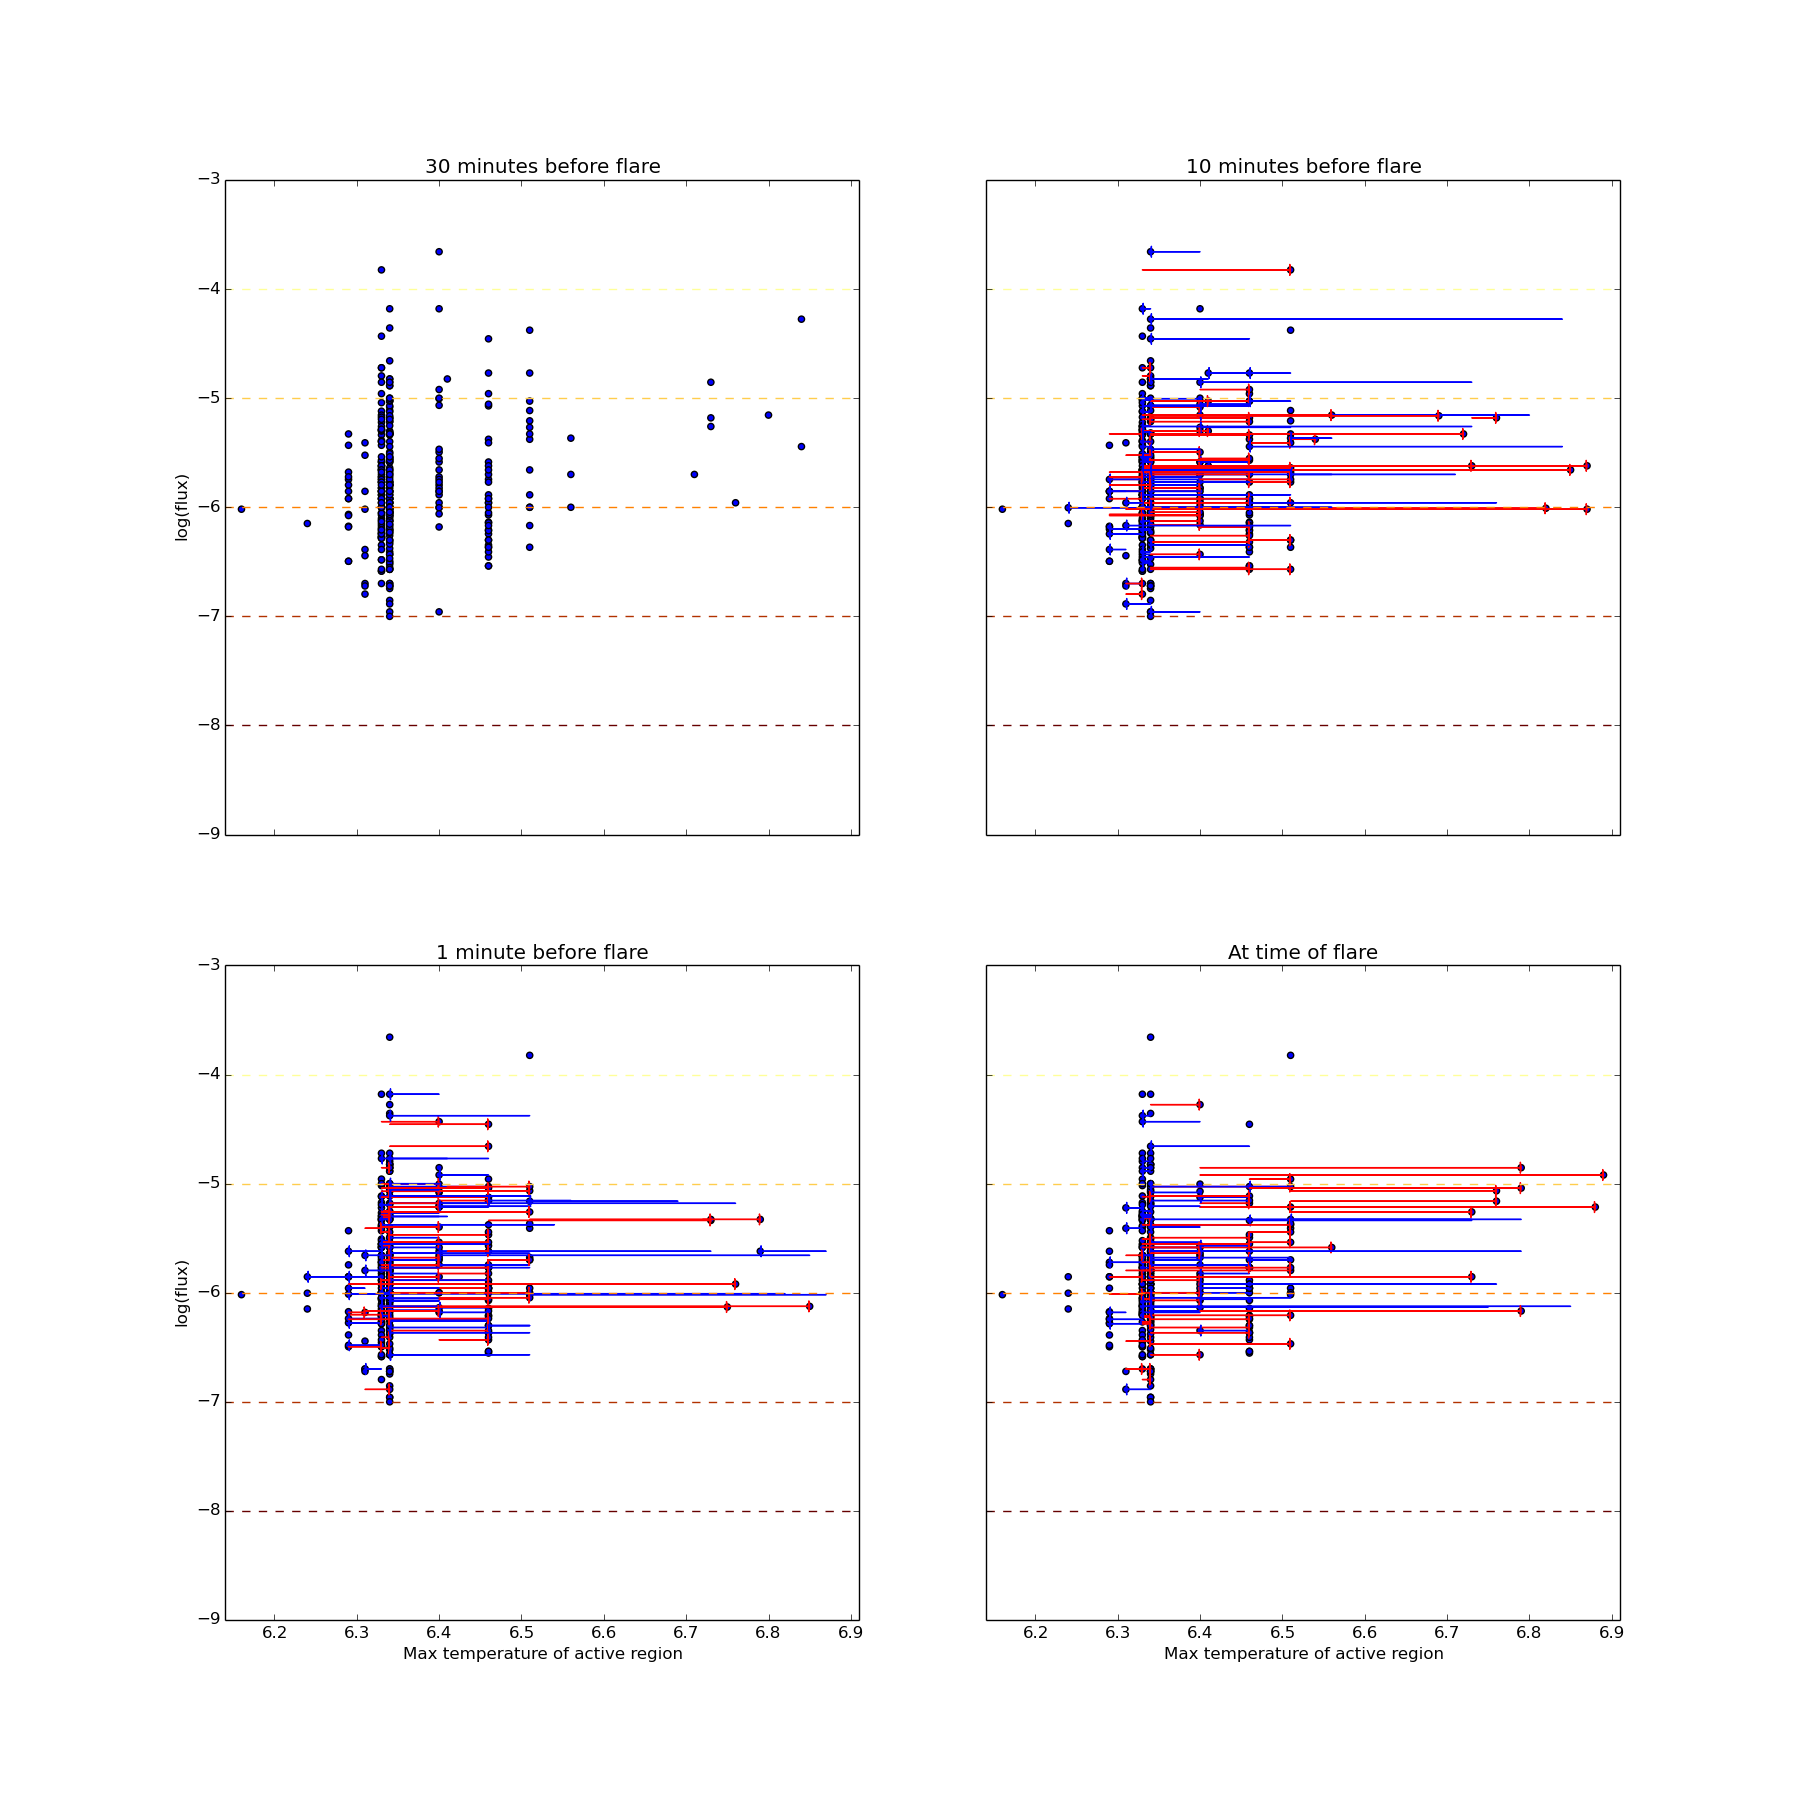
\includegraphics[width=0.9\columnwidth]{tempplotsmax/allflares.png}
	\caption{Scatter graph of flare peak flux against 5th percentile temperature of the corresponding active regions for the same four times as in Figure \ref{fig:allflares_max}.}
	\label{fig:allflares_p5}
\end{figure}
\begin{figure}
	\centering
		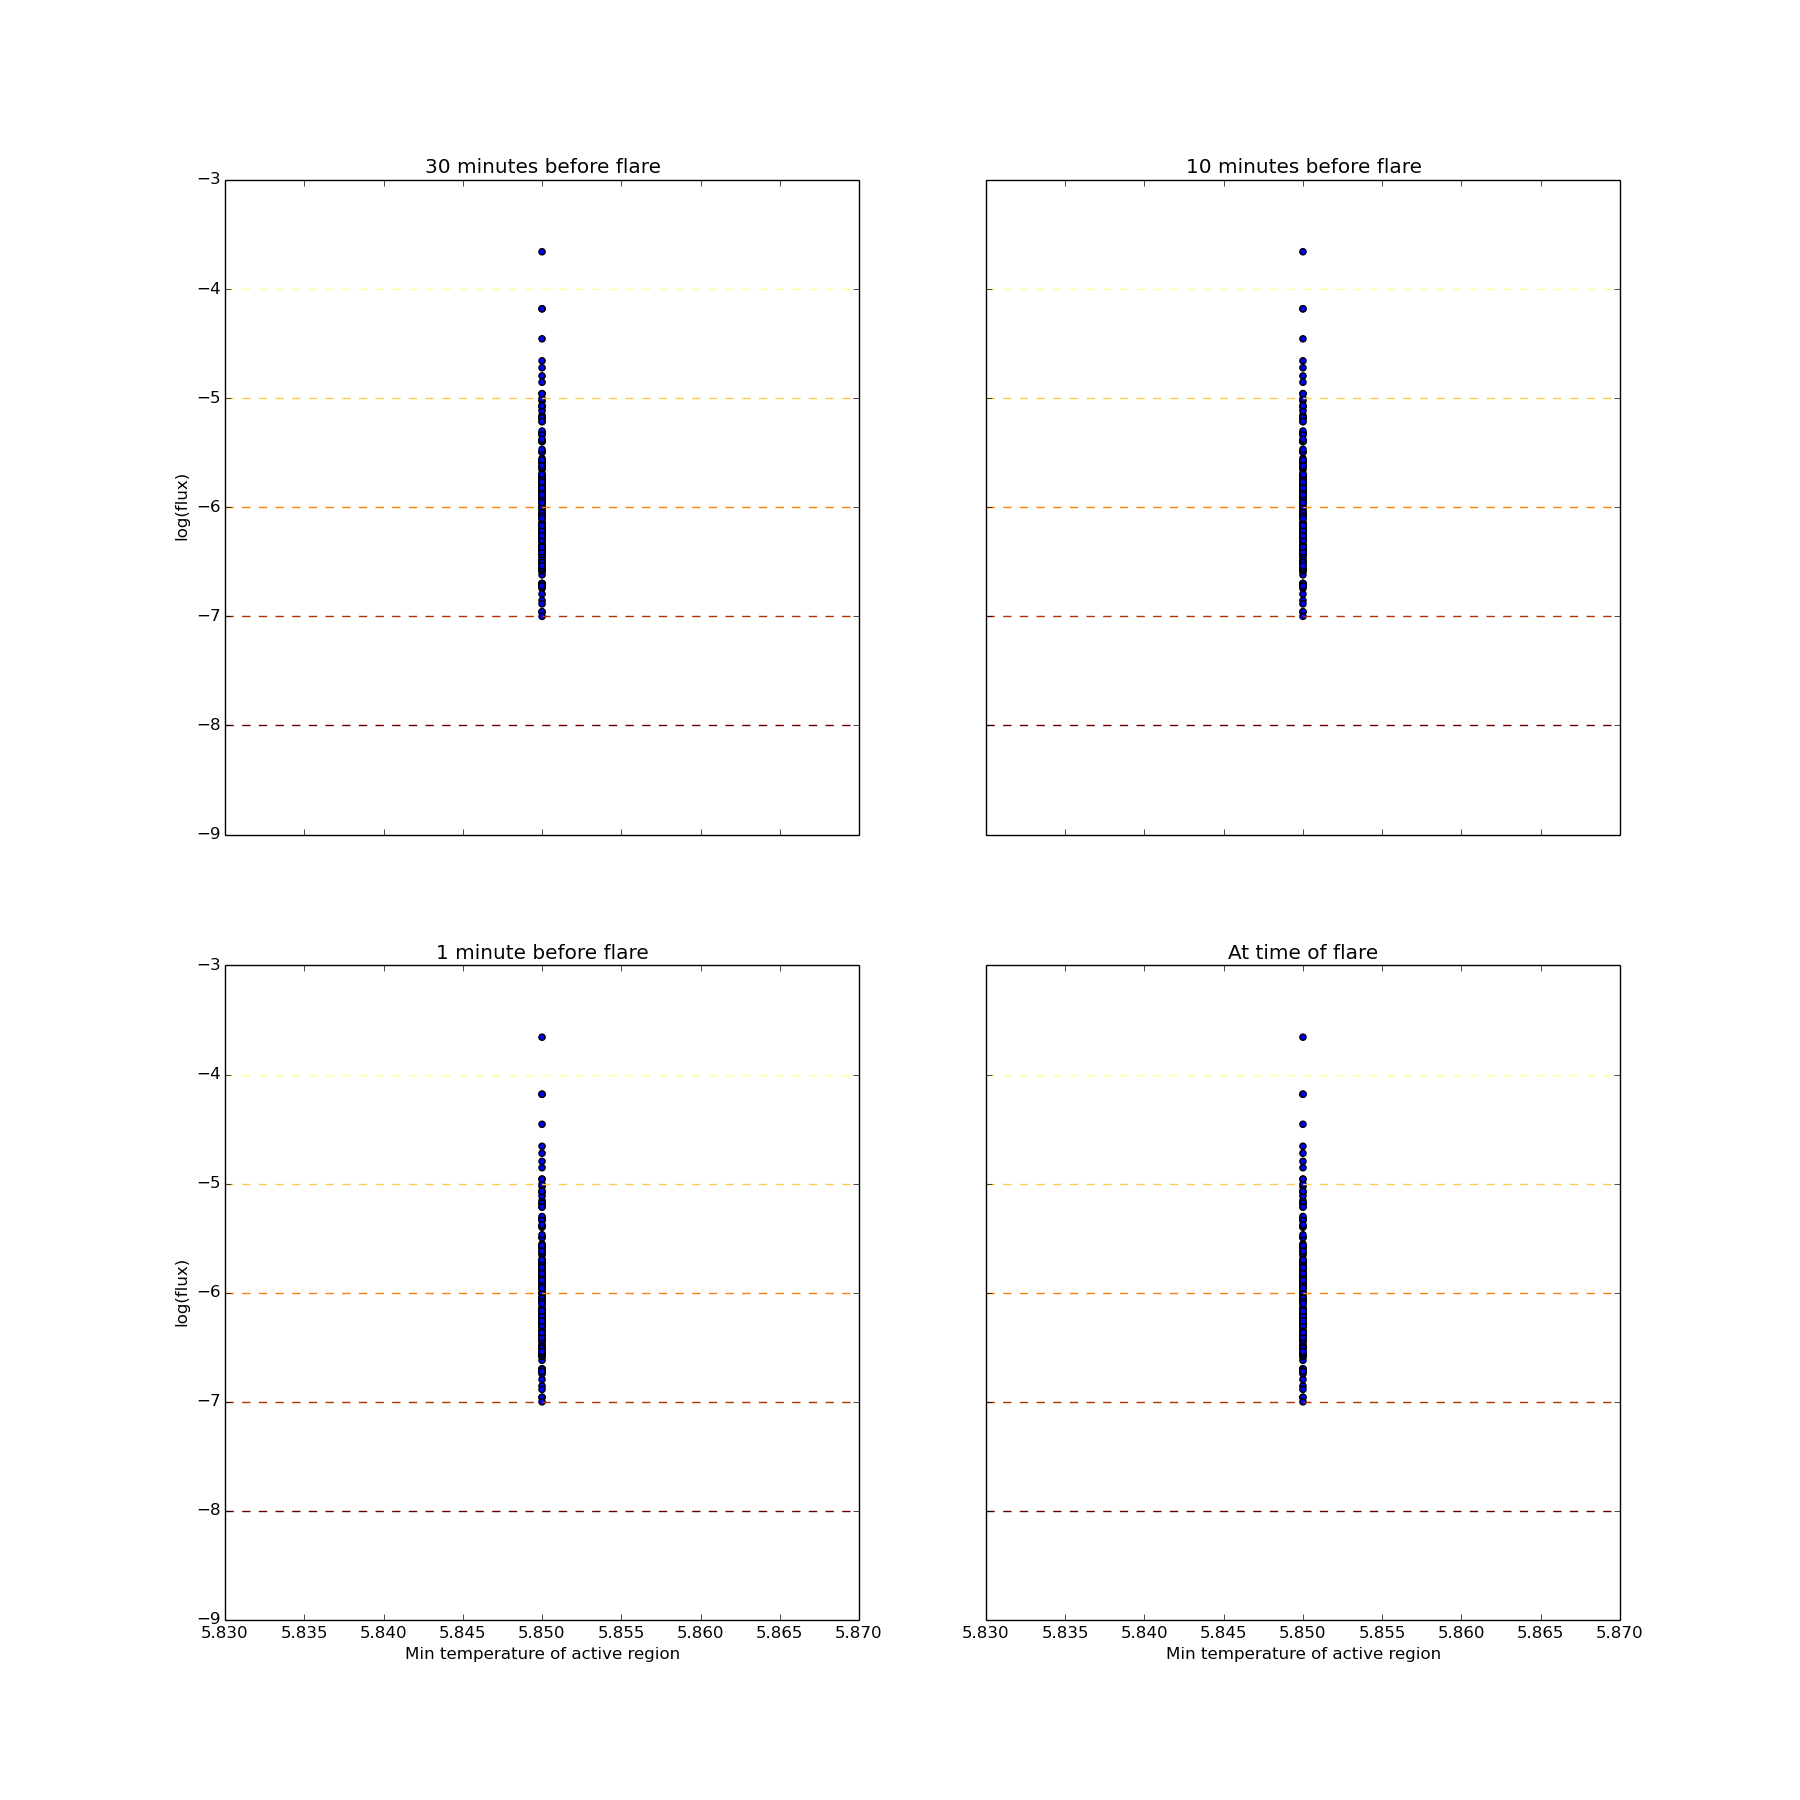
\includegraphics[width=0.9\columnwidth]{tempplots_min/allflares.png}
	\caption{Scatter graph of flare peak flux against minimum temperature of the corresponding active regions for the same four times as in Figure \ref{fig:allflares_max}.}
	\label{fig:allflares_min}
\end{figure}


%===========================================================================
\section{Discussion and conclusions}
From this study, it appears that there is no clear link between solar flares and coronal temperatures.
This is probably mostly due to the relatively small number of flares studied - a much larger sample size would have to be used to properly determine any link or lack thereof.
However, this work does demonstrate that it is now possible to study temperature distributions of the corona in high resolution and on short timescales using fast temperature analysis tools such as that described in Paper 1.

\subsection{Long-term temperature distribution}
Figures 1 and 2 show that there is no clear trend in the long-term temperature distribution before flares occur.
This is also the case for the other active regions investigated. If any trend in temperature does occur before large flares, it may be on a shorter timescale than investigated here, and may only be noticable for very large flares.
Any further work on this topic should therefore look at shorter timespans with higher cadence, and perhaps only consider active regions associated with X-class flares.

\subsection{Temperatures of active regions before flares}
From figure 3 it can be seen that there does appear to be some grouping of flaring active regions into groups of temperatures, and that a few of the larger flares are associated with active regions at higher temperatures than most of the other flares investigated.
However, no clear correlation can be seen between peak flare flux and active region temperature.
A much larger sample of flares is needed in order to properly determine whether or not a link exists between the two.

%===========================================================================
\section*{Acknowledgements}

%===========================================================================
\section*{annexes}

%===========================================================================
\bibliographystyle{plainnat}
\bibliography{C:/Users/Drew/Dropbox/Thesis/thesis_refs,C:/Users/Drew/Documents/library}

\end{linenumbers}
\end{document}